%#!platex manual; latexml --noparse --destination=./manual.xml manual.tex; latexmlpost --format=xhtml --destination=./html/manual.xhtml --split  --novalidate manual.xml
\documentclass{jbook}
\usepackage{a4}
\usepackage{latexsym}
\usepackage{url}
\usepackage{epsfig}
\oddsidemargin 0in
\evensidemargin 0in
\date{平成24年4月6日}
\newcommand{\smlsharp}{SML\#}

\newcommand{\version}{1.00}
\newcommand{\smlsharpSize}{30万}
%%%%% set the following!
\newcommand{\authors}{}

\newcommand{\func}{\rightarrow}
\newcommand{\vbar}{\mbox{\ |\ }}
\newcommand{\code}[1]{\mbox{{\tt #1}}}
\newcommand{\nonterm}[1]{\mbox{$\langle$}{\it #1}\mbox{$\rangle$}}
\newcommand{\sep}{\mbox{\ \ }}

\newenvironment{program}{\begin{tt}\begin{quote}}{\end{quote}\end{tt}}
% \newcommand{\myem}{\ \ \ \ \ \ \ }
\newcommand{\myem}{\ \ \ \ \  }
\newcommand{\myfm}{ \ \ \ \ \ }


\title{プログラミング言語\smlsharp{}解説}
\author{
\authors
\\
東北大学 電気通信研究所
}


\begin{document}
\maketitle

\tableofcontents

% \part{はじめに}
\chapter*{はじめに}

	本書は東北大学電気通信研究所で開発された関数型プログラミング
言語\smlsharp{}の公式ドキュメントです.
	\smlsharp{}の概要,プログラミングチュートリアル,および,参照マ
ニュアルの役割をはたす総合ドキュメントを意図しています.
	現在の第\version{}版には参照マニュアルは含まれまれず,MLプログラ
ミングのチュートリアルも一部未完成ですが,関数型言語に慣れた人はもちろん
これからプログラミングを始めようとする人も,\smlsharp{}言語を使って高度
なプログラミングを書き始めるために十分な情報を含んでいるはずです.
	特に,第\ref{part:tutorial}部のチュートリアルは,関数型言語の
基本的な考え方やMLプログラミングの基礎を含んでおり,ML言語の手軽な教科書
としても使用できます.
	ML言語をより本格的に学ぶには,Standard MLの教科書
\cite{ohori00sml}や大堀によるその他のMLの解説
\cite{ohor95jssst,ohor94ipsj}を参照ください.

	\smlsharp{}は,これら教科書で書かれたStandard MLと後方互換性のあ
る言語です.
	ネイティブコードコンパイラですが,対話型プログラミングもサポート
しており,だれでも手軽にMLプログラミングを楽しむことができます.
	さらに,\smlsharp{}が実現しているC言語とのシームレスな連携などの
機能は,高度で信頼性の要求される本格手にな実用的システムの開発にも威力を
発揮すると信じています.

	本ドキュメントを参考に,\smlsharp{}プログラミングをお楽しみくだ
さい.
	不明な点や要望等は著者にご連絡ください.

	この文書は,現在\LaTeX{}とLaTeXMLを用いて作成しています.
	表示にはMathMLのレンダリングが可能なブラウザが最適です.
	現時点では,FireFoxが対応しています.

\begin{flushright}
2012年4月\\
東北大学電気通信研究所\\
\authors
\end{flushright}

\part{概要}
\label{part:outline}

\chapter{\smlsharp{}の概要}
\label{chap:intro}

	本章では\smlsharp{}言語の概要を説明します.

\section{\smlsharp{}とは?}
\label{sec:whatIsSmlsharp}

	\smlsharp{}は,以下のような特徴をもったML系関数型プログラミング言語です.
\begin{enumerate}
\item {\bf Standard MLとの後方互換性.}
	\smlsharp{}は,ML系言語の標準の厳密な仕様であるStandard
MLとの完全な後方互換性をもっています.
	Standard MLの形式的な仕様\cite{sml}をみたすすべてのプログラムを
コンパイルできます.

\item {\bf レコード多相性.}
	レコード多相性\cite{ohor95toplas}は,オブジェクトやデータベース
のタプルなどに現れるラベル付きレコードをML言語に完全に統合するために必要
な型システムの機能です.
	\smlsharp{}は,この機能を完全にサポートしています.

\item {\bf SQLのシームレスな統合.}
	SQLはデータベースの標準問い合わせ言語であり,データベースを利用
するプログラムで必ず必要となる機能です.
	\smlsharp{}は,SQLの一部の機能をライブラリとして提供するのでは
なく,SQLそのものを多相型をもつ型第一級の式として統合しています.
	この機能により,複雑なプログラムデータベース操作を,MLプログラム
の中で直接プログラムすることができます.
	
\item {\bf C言語との直接連携.}
	システムプログラミングを含む種々のOSの機能の利用にはC言語で記述
されたライブラリのアクセスが必要となります.
	\smlsharp{}では,名前を外部名宣言するだけで,C言語で書かれCコン
パイラでコンパイルされた関数を呼び出すことができます.

\item {\bf マルチコアCPU上のネイティブスレッドのサポート.}
	\smlsharp{}の並行かつオブジェクトを動かさないGCの機能により,
C言語との連携機能を使い,OSのスレッドライブラリを直接呼び出すことができ
ます.
	従って,OSがマルチコアCPU上での並列実効をサポートしさえすれば,
スレッドを使った高水準なMLプログラムを書き,マルチコアCPU上で効率良く実
効することができます.

\item {\bf 分割コンパイルとリンク.}
	\smlsharp{}は,従来のインクリメンタルなコンパイルではない,真の分
割コンパイルを実現しています.
	各モジュールのインターフェイスの確定後は,各モジュールを独立に開
発しコンパイルやテストできます.
	さらに,\smlsharp{}コンパイラは,分割コンパイルの対象となる各ソー
スコードを,システム標準のELFフォーマットに従うオブジェクトファイルにコ
ンパイルし,システムのリンカーでCのライブラリなどとともにリンクします.
	この機能により,C言語やSQLなどを使う大規模プログラムを安全かつ効
率的に開発です.

\end{enumerate}
	
	\smlsharp{}コンパイラおよび実行時処理系は,東北大学電気通信研究
所大堀研究室で開発され,東北大学が著作権保有するオープンソースソフトウエ
アです.
	BSDスタイルの\smlsharp{}ライセンス(\ref{sec:smlsharpLicence}節参照)に
よって公開されており,だれでも自由に利用することができます.
	このライセンスは,二次著作物(つまりコンパイラで作成されたシステ
ムなど)に関する制限の少ないフリーソフトウェアライセンスであり,企業の商
品開発にも安心して使用できます.

\section{\smlsharp{}ライセンス}
\label{sec:smlsharpLicence}

Copyright (c) 2006 - 2012, Tohoku University.\\
All rights reserved.\\

Redistribution and use in source and binary forms, with or without
modification, are permitted provided that the following conditions are
met:

\begin{itemize}
\item 
  Redistributions of source code must retain the above copyright
  notice, this list of conditions and the following disclaimer. 
\item 
  Redistributions in binary form must reproduce the above
  copyright notice, this list of conditions and the following disclaimer
  in the documentation and/or other materials provided with the
  distribution. 
\item 
  Neither the name of Tohoku University nor the names of its
  contributors may be used to endorse or promote products derived from
  this software without specific prior written permission.  
\end{itemize}

THIS SOFTWARE IS PROVIDED BY TOHOKU UNIVERSITY AND CONTRIBUTORS "AS IS"
AND ANY EXPRESS OR IMPLIED WARRANTIES, INCLUDING, BUT NOT LIMITED TO,
THE IMPLIED WARRANTIES OF MERCHANTABILITY AND FITNESS FOR A PARTICULAR
PURPOSE ARE DISCLAIMED. IN NO EVENT SHALL TOHOKU UNIVERSITY OR
CONTRIBUTORS BE LIABLE FOR ANY DIRECT, INDIRECT, INCIDENTAL, SPECIAL,
EXEMPLARY, OR CONSEQUENTIAL DAMAGES (INCLUDING, BUT NOT LIMITED TO,
PROCUREMENT OF SUBSTITUTE GOODS OR SERVICES; LOSS OF USE, DATA, OR
PROFITS; OR BUSINESS INTERRUPTION) HOWEVER CAUSED AND ON ANY THEORY OF
LIABILITY, WHETHER IN CONTRACT, STRICT LIABILITY, OR TORT (INCLUDING
NEGLIGENCE OR OTHERWISE) ARISING IN ANY WAY OUT OF THE USE OF THIS
SOFTWARE, EVEN IF ADVISED OF THE POSSIBILITY OF SUCH DAMAGE.

\section{ML言語について}
\label{sec:mllanguage}

	\smlsharp{}はML系関数型プログラミング言語の一つです.
	本節では\smlsharp{}の理解のためにML言語の概要を説明します.

	ML言語はEdinburgh LCF\cite{gord79}のメタ言語({\bf M}eta {\bf
L}anguage)として開発されました.
	メタ言語とは,ある言語の分析や記述をするための言語のことです.
	プログラミング言語を変換したり処理するための言語もメタ言語とみな
すことができます.
	Edinburgh LCFは計算可能な関数(つまりプログラム)を対象とした一
種の定理証明システムであり,その対象となる関数はPPLAMBDAと呼ばれる型付ラ
ムダ計算で表現されました.
	LCF MLはPPLAMBDのメタ言語,つまりPPLAMBDで書かれたプログラムを操
作しするためのプログラミング言語でした.
	MLの名前はこの歴史的事実に由来しています.
	関数を表すラムダ式を柔軟に操作する目的のために,ML自身ラムダ計
算を基礎とする関数型言語として設計されました.
	さらにプログラムを操作するプログラムを柔軟にかつ信頼性を持って記
述するために,型の整合性を自動的に検査する型推論機構が初めて開発されまし
た.

	このLCF MLは,PPLAMBDAの操作言語にとどまらない汎用のプロ
グラミング言語として価値があることが認識され,CardelliによってLCFとは独
立したプログラミング言語としてのMLコンパイラが開始され,PDP11やVAX VMSな
どの上に実装され使用されました.
	その後,Milner,Harper,MacQueen等によってプログラミング言語とし
ての仕様策定の努力がなされ,さらにこの言語がEdinburg大学によってCardelli
のML上に実装されました.
	これらの成果を踏まえ,Standard MLの仕様\cite{sml}が確定し,その
後改訂され現在のStandard ML言語仕様\cite{sml97}として完成しました.

\section{\smlsharp{}の歴史}
\label{sec:smlsharpHistory}

	1993年,沖電気工業(株)関西総合研究所にて,大堀により,Standard
ML of New Jerseyコンパイラに多相型レコード演算を加え拡張したプロトタイプ
SML\# of Kansaiが開発されました.
	その時の\smlsharp{}のtypesメーリングリストへのアナウンスは,今で
もインターネット上に記録されています
(
\url{http://www.funet.fi/pub/languages/ml/sml%23/description}
).
	SML\# of Kansaiの名前は,このコンパイラにて初めて多相型が与えら
れたレコード演算子"\code{\#}"を象徴するものです.
	このコンパイラは,その後に出版されたACM TOPLASの論文
\cite{ohor95toplas}にて,``\smlsharp{}''の名前で紹介されています.


	2003年に,北陸先端科学技術大学院大学にて,文部科学省リーディング
プロジェクトe-Society基盤ソフトウェアの総合開発「高い生産性をもつ高信頼
ソフトウエア作成技術の開発」
(
\url{http://www.tkl.iis.u-tokyo.ac.jp/e-society/index.html}
)
(領域代表者:片山卓也)
の一つの課題
「プログラムの自動解析に基づく高信頼ソフトウェアシステム構築技術」(2003年―2008年,究代表者:大堀 淳)
として,
次世代ML系関数型言語\smlsharp{}をスクラッチから開発するプロジェクトを開始しました.

2006年4月,プロジェクトは,大堀とともに東北大学電気通信研究所に移り開発
を継続しています.

2008年のe-Societyプロジェクト終了後も,東北大学電気通信研究所大堀研究室
にて,\smlsharp{}の研究開発を続けています.
	
\section{\smlsharp{}開発チームと連絡先情報}
\label{sec:smlsharpTeam}

	現在(2012年4月)\smlsharp{}は,
\begin{itemize}
\item 
大堀 淳(東北大学電気通信研究所)
\item 
上野雄大(東北大学電気通信研究所)
\end{itemize}
の2名が,大学院大学院情報科学研究科の大堀研究室に所属の大学院生の協力の
下,開発を行なっています.

	\smlsharp{}のこれまでの主な開発者は以下の通りです.
	(敬称は略させていただいています.
	所属は\smlsharp{}の開発に携わった時のものです.)
\begin{itemize}
\item 大堀 淳(北陸先端科学技術大学院大学情報科学研究科,東北大学電気通信研究所)
\item 大和谷 潔(算譜工房)
\item Nguyen Huu Duc(北陸先端科学技術大学院大学情報科学研究科,東北大学電気通信研究所)
\item Liu Bochao(北陸先端科学技術大学院大学情報科学研究科,東北大学電気通信研究所)
\item 纓坂 智(北陸先端科学技術大学院大学情報科学研究科)
\item 上野雄大(北陸先端科学技術大学院大学情報科学研究科,東北大学電気通信研究所)
\end{itemize}

	東北大学電気通信研究所では,\smlsharp{}に関する情報共有の目的で
以下のwebサイトやメーリングリストを管理しています.
\begin{itemize}
\item \smlsharp{}ホームページ.
\url{http://www.pllab.riec.tohoku.ac.jp/smlsharp/ja/}
コンパイラや本書を含む文書の最新版などもここからダウンロードできます.

\item \smlsharp{}メーリングリスト.
{\tt smlsharp-list@pllab.riec.tohoku.ac.jp}
\smlsharp{}に関する一般的な議論や情報交換のためのメーリングリストです.
使用言語は日本語または英語です.投稿は購読者のみ行うことができ,投稿され
た全てのメールはWeb上に公開されます.\\
参加方法:\url{http://www.pllab.riec.tohoku.ac.jp/mailman/listinfo.cgi/smlsharp-list?language=ja}\\
アーカイブ:\url{http://www.pllab.riec.tohoku.ac.jp/pipermail/smlsharp-list/}

\item \smlsharp{}開発者への連絡メールアドレス.
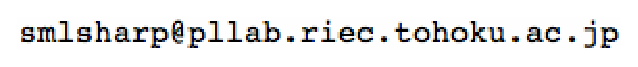
\epsfig{file=smlsharp-list.eps,width=0.4\textwidth}
共同研究の提案や各種問い合わせなどにご利用ください.
\end{itemize}

\section{謝辞}
\label{sec:acknowledgements}

	2003年にスタートした\smlsharp{}開発の過程では,以下を含む色々
なご指導やご協力を頂きました.
	ここに謝意を表します.
	
\subsection{プロジェクトファンディング}
	\smlsharp{}言語の研究開発は,2003年から5年間の文部科学省リーディ
ングプロジェクトe-Society基盤ソフトウェアの総合開発「高い生産性をもつ高
信頼ソフトウエア作成技術の開発」の一つの課題
「プログラムの自動解析に基づく高信頼ソフトウェアシステム構築技術」(究代
表者:大堀 淳)としてスタートをきることができました.
	このプロジェクトの主要な目標が\smlsharp{}言語コンパイラの開発で
した.
	\smlsharp{}は開発ソースの総量が\smlsharpSize{}行を超える大規模シ
ステムです.
	このプロジェクトの支援がなければ,\smlsharp{}の開発は困難であっ
たと思われます.
	文部科学省,e-Societyの領域代表の片山卓也先生,および関係各位に
深謝いたします.

\subsection{\smlsharp{}が使用しているソフトウエア}

	\smlsharp{}言語は,第\version{}版以降は,\smlsharp{}自身でコンパ
イルし開発を行なっていますが,それ以前は,Standard ML of New Jerseyおよ
びMLTonのStandard MLコンパイラを使って開発を行いました.

	\smlsharp{}は前節(\ref{sec:smlsharpTeam})の開発チー
ムによって開発されたソフトウェアです.
	\smlsharp{}言語と一部C言語による約\smlsharpSize{}行に登るソース
コードの殆どをスクラッチから開発しましたが,一部に以下のコードを利用して
います.

\begin{center}
\begin{tabular}{|c|c|c|}
\hline
内容 & \smlsharp{}ソース上の位置 & ソース
\\\hline
ML-Yacc & src/ml-yacc  & Standard ML of New Jersey (110.73)
\\\hline
ML-Lex & src/ml-lex  & Standard ML of New Jersey (110.73)
\\\hline
2分探索木関数 & src/smlnj-lib &  Standard ML of New Jersey (110.73)
\\\hline
IO,POSIX IO
ファイルパス関数
&
src/smlnj/Basis
&
Standard ML of New Jersey (110.73)
\\\hline
浮動小数点/
文字列変換関数
&
src/runtime/netlib
&
the Netlib
\\\hline
SMLFormatの
SML文法定義
&
src/smlformat/generator/main/
&
Standard ML of New Jersey
\\\hline
\end{tabular}
\end{center}
	これらソースは,いずれも\smlsharp{}ライセンスと整合性あるライセ
ンスで配布されているオープンソースソフトウエアです.
	「\smlsharp{}ソース上の位置」にそれぞれのライセンスが添付されて
います.


\subsection{研究開発協力者}
	\smlsharp{}言語の開発にあたっては,多くの人々からの指導を受けま
した.
	過去現在の開発チーム(第(\ref{sec:smlsharpTeam})節)以外で特に
貢献のあった方々は以下の通りです.
\begin{itemize}
\item 篠埜功氏.
大堀と共に,関数フュージョン機能を持つ新たしいインラインの理論および
その実験的な実装を行いました.
	この機能は実験的な実装がありますが,まだ十分な完成度が得られてお
らず\smlsharp{}\version{}版に組み込まれていませんが,将来取り入れたいと
考えています.
\item 大友聡顕氏.
	大堀,上野と共に,オブジェクトを動かさないGCの研究開発に携わり,
初期の実験的な実装を行い,この方式が有望であることを確認しました.
	この成果は,現在のオブジェクトを動かさないGCの方式の開発と実装の
契機となったものです.
\end{itemize}
	これらの方々以外にも,\smlsharp{}は,大堀等との共同で行なった様々
な型理論やコンパイル方式の基礎研究を基に設計されています.
	現在の\smlsharp{}言語に直接生かされている出版された基礎研究成果
には以下のものが含まれます.
\begin{itemize}
\item レコード多相性の理論\cite{ohor92popl,ohor95toplas}.
\item データベースの型推論\cite{ohor88lfp}.
\item データベース言語(Machiavelli)\cite{ohor89sigmod,bune96tods}.
\item ランク1多相性の型理論\cite{ohor99icfp}.
\item MLのunboxed意味論\cite{ohor97unbox}.
\item MLにおける自然なデータ表現\cite{nguyen06ppdp}.
\item オブジェクトを動かさないGC\cite{ueno11icfp}.
\item 軽量の関数融合\cite{ohor07popl}.
\end{itemize}
	それ以外にも多くの共同研究者から色々な機会に示唆や助言を頂いてお
り,それらは1989年にまで遡りますが,それらの方々の列挙は割愛させてい
ただきます.


\section{\smlsharp{}第\version{}版の機能と制限}

	我々開発チームは第\ref{sec:whatIsSmlsharp}節でのべた機能をすべて
開発し\smlsharp{}開発開始時に目標とした機能を実現しています.
	第\version{}版にその殆どが含まれていますが,以下の制約があります.
\begin{enumerate}
\item マルチスコア上のネイティブスレッド.
	この機能は現時点では,十分にテストされていないため,デフォルトで
はオフになっています.
	システム構築時({\tt ./configure}時)に{\tt --enable-thread}
を指定すればオンになり,コンパイラはネイティブスレッド対応のコードを生成
します.
	OSのスレッドライブラリを{\tt \_import}すれば,マルチコア上でネイ
ティブスレッドが動くはずです.

\item データベースサーバ.
	現在デフォルトでサポートされているデータベースサーバは
PostgreSQLのみです.
	MySQLも接続できることを確認しています.
	近い将来,数のサーバへの接続機能および実行時の複数のサーバの同時
使用のサポートを行う予定です.

\item ターゲットアーキテクチャ.
	現在の\smlsharp{}コンパイラは,32ビットのインテルアーキテクチャ
(x86, IA-32)向けのコード生成器しかもっていません.
	将来,マルチターゲット化を行う予定です.
	特に,インテルの64ビット版への対応は,近い将来行う予定です.

\item Windows版の対話型ループの制約.
	\smlsharp{}\version{}版は,すべて一つのネイティブコードコンパイ
ラで動いています.
	対話型ループも,(1)ユーザ入力のコンパイル,(2)現在のコンパイラにリンク,
(3)動的にロード,のサイクルによって実現されています.
	この中で(2)のリンクをWindowsシステム上で実現するためには,シ
ステムの制約上,これまでに作られたオブジェクトファイル毎にリンクのための
ファイルをコマンドラインで指定する必要があります.
	このファイル数が,対話型環境での入力に従って増えて行きます.
	そのため,Windows上の対話型環境の連続使用は,コマンドラインの最
大文字数によって制約されます.
\end{enumerate}

% \section{第1章の用語解説及ぶFAQ}
% \label{sec:glossary1}
% 
% \begin{description}
% \item[BSDスタイルライセンス] 
% 二次著作物に関する制限が少ないオープンソースソフトウエアライセンスの一つ.
% 
% BSDスタイルライセンスでは,ライセンス内容をドキュメント等に表示する限り,
% ソースおよびバイナリ形式をとわず,コードの使用,変更,再配布を認めている.
% これにより,二次著作物,つまりそのソフトを利用して作成される種々の製品を,
% 自由に作成し配布や販売することができる.
% 
% 正確にな内容は英文のBSDライセンス(BSD License,Berkeley Software
% Distribution License)を参照.
% 
% 
% \item[メタ] 
% 「後に」あるいは「越えて」といった位置を表すギリシャ語.
% この接頭語を含むギリシャ語metaphsicaがアリストテレスのよって書かれた名前
% の付けられなかった本の題名の代わに使われることによって,
% 「「自然学」の後に位置する本」という意味のmetaphsicaが,
% その本の内容である「哲学,形而上学(metaphisics)」
% を意味する用語として定着した.
% それに伴い,もともとの位置の概念であったmetaに,自然学を超越する
% という意味が与えられ,種々の分野で使用されようになった.
% たとえば言語学の分野では,metaは,通常の言語の使用を分析するために用いる
% 言語として使用される.
% \end{description}
% 
% FAQ:
% \begin{itemize}
% \item 
% {[Q]} \smlsharp{}の開発に参加したいのですが?\\
% {[A]} もちろん可能です.意欲のある方はご連絡ください.一緒にプログラミング
% 言語の色々な機能を実現していきましょう.今後,研究室以外の人々とのソース
% の共有や変更の管理等の体制を整えていく予定です.
% 
% \item  
% {[Q]} 東北大学電気通信研究所でプログラミングを学ぶことができますか?\\
% {[A]} 東北大学電気通信研究所の不タッフ(教授,准教授,助教)は,学部は工学
% 部,大学院は情報科学研究科または工学研究科大学院の教員を兼務し,工学部知
% 能情報システム総合学科の学部4年生,および教員の所属する情報科学研究科お
% よび工学研究科大学院の学生を受け入れています.大堀研究室は情報科学研究科
% の教員を兼務しています.
% 
% 学部の場合は,工学部知能情報システム総合学科に,大学院なら情報科学研究科
% に入学し大堀研究室を志望すれば,我々と一緒に\smlsharp{}やその他プログラ
% ミング言語及びデータベースの研究開発を思う存分行うことができます.
% 
% \end{itemize}

\part{チュートリアル}
\label{part:tutorial}

\chapter{\smlsharp{}プログラミング環境の準備}
\label{chap:tutorialEnvironment}

	第2部では,\smlsharp{}でプログラミングをマスターするための
チュートリアルを提供します.

	まず\smlsharp{}プログラミング環境をととのえましょう.

\section{Unix系OS,Emacsエディタ,その他ツールの整備}
\label{sec:tutorialEnvironmemt}

	プログラミングのためには,
\begin{itemize}
\item 使いやすい高機能エディタ
\item コンパイラとリンカー
\end{itemize}
を含むプログラミング環境が必要です.
	\smlsharp{}でのプログラミングに必要とされるプログラミング環境は,
\smlsharp{}コンパイラのインストールを除けば,C言語の場合と同様です.
	Javaなどの言語では,これらを統合した対象言語に特化したEclipsなど
の統合開発環境を使用する場合が多いですが,Cとの直接連携機能を用いたシス
テムプログラミングやSQLを使ったデータベース操作などの\smlsharp{}の先端機
能を駆使したプログラミングを十分に楽しむためには,以下のような標準的なプ
ログラミング環境を整えることを勧めます.

\begin{description}
\item[Unix系のOS] 
	高度なプログラム開発には,Linux,FreeBSD(Mac OCを含む)等のUnix
系OSが豊富なツールを含んでいて便利です.
	Windows系のOSがインストールされたPCの場合は,VMWareなどの仮想マ
シンを利用してLinuxなどの環境を容易に構築できます.
	Windows系OSでは,Cygwinでもほぼ同等の環境が得られます.
	Windows系OSで,Emacsが自由に使いこなせれば,MinGW(+MSYS)でも十
分にプログラミングを楽しむことができると思われます.
	

\item[Emacsエディタ]
	プログラミングにもっとも適したエディタの一つです.
	プログラミングは,テキスト形式の文を書き,コンパイルしテストをし,
修正する,という作業の繰り返しであり,その大部分の時間はテキストエディタ
との付き合いとなります.
	そこで,強力でカスタマイズ可能なテキストエディタの選択が重要です.
	Emacs系テキストエディタ(GNU EMACS,XEMACSなど)は,複数のバッファ
の操作,ディレクトリなどのファイルの管理,コンパイラなどのコマンド起動,
さらに,それらの柔軟なカスタマイズ機能を備えた強力なエディタであり,プロ
グラミングやLaTex文書などの複雑で高度な文書の作成に最適なエディタです.
	使い始める時に少々練習が必用ですが,使いこなせば,プログラム開発
の強力な道具となります.
	Unix系OSでは通常インストール済みです.

\item[Cコンパイラ] 
	\smlsharp{}コンパイラは,x86アーキテクチャのネイティブコードにコ
ンパイルし,ソースコードをOS標準のオブジェクトファイルを作成し,さらに
それらをリンクし実行形式ファイルを作成します.
	この過程でGNU Cコンパイラ{\tt gcc}を通してリンカーを呼び出します.
	Unix系OSやCygwin,MinGWのインストール時にプログラム開発用に適し
たシステムを選択すれば標準でインストールされているはずです.

	\smlsharp{}プログラムのみをコンパイルしリンクする場合は,ユーザ
が直接{\tt gcc}コンパイラを呼び出す必要はありませんが,C言語との直接連携
機能を使いより高度なプログラミングを行うためにも,{\tt gcc}コンパイラに
慣れておくことをお勧めします.

\item[データベースシステム] 
	\smlsharp{}のデータベース機能を使用すにはデータベースシステムを
インストールする必要があります.
	第\version{}版では,PostgreSQLがインストール時バインドされます.
	データベースアクセス機能を使用するには,PostgreSQLをインストール
する必要があります.
	詳細はOSに依存しますが,いずれの場合も簡単にインストールできるは
ずです.
\end{description}

	次節(\ref{sec:tutorialInstall})で説明する通り,Windowsのユーザ
に対しても,コンパイル済みのバイナリープログラムを用意しています.
	このバイナリを使用すれば,WindowsOSのアプリケーションの一つ
とすて\smlsharp{}コマンドが使用可能になります.
	その場合でも,Windows上にEmacsをインストールすることをおすすめし
ます.
	Emacsが持つshell機能をを使えば,\smlsharp{}コンパイラだけでも,
十分にに本格的な\smlsharp{}言語のプログラムを楽しむことができるはずです.

\section{\smlsharp{}コンパイラの構造とブートストラップ}
\label{sec:tutorialInstall}

	この節は,\smlsharp{}コンパイラをインストールし使用する上で,理
解する必要はありませんが,やや時間がかかる\smlsharp{}コンパイラのインス
トール処理の理解や,さらにコンパイラの一般的な構造を理解する上で有用と思
います.

	\smlsharp{}\version{}版コンパイラは,\smlsharp{}言語で書かれた
ファイルを分割コンパイルし,インテルのIA-32ネイティブコードを生成します.
	対話型モードも,このコンパイラを使い,
(1)現在の環境下で分割コンパイル,
(2)システムとのリンク,
(3)オブジェクトファイルの動的ロード
を繰り返すことによって実現しています.
	\smlsharp{}言語とCで書かれており,さらにコンパイラは,自分自身の
コンパイル時に以下のツールを使用しています.
\begin{itemize}
\item ml-lex,ml-yacc.字句解析および構文解析ツール.
\item SMLFormat.プリンタ自動生成ツール
\item 基本ライブラリ
\end{itemize}
	これらも\smlsharp{}言語で書かれています.

	\smlsharp{}コンパイラは,各\smlsharp{}ファイル(Standard MLファ
イルを含む)をシステム標準のオブジェクトファイルにコンパイルします.
	コンパイルしたファイルは,システム標準のリンカーやアセンブリプロ
グラムによって実行形式ファイルに変換できます.
	従って,\smlsharp{}コンパイラは,C言語のコンパイラと\smlsharp{}
コンパイラがあれば構築できます.
	しかし,もちろん,\smlsharp{}コンパイラを初めてインストールする
時には,\smlsharp{}コンパイラはまだ存在しません.
	このブートストラップの問題を解決し,\smlsharp{}を構築する標準の
手順は以下のとおりです.

\begin{enumerate}
\item \smlsharp{}コンパイラのソースコードをコンパイルするのに十分なコマ
ンド(minismlsharp)を作るためのアセンブリファイルを用意.

\item インストールするシステムの下で,minismlsharpのアセンブリファイルを
アセンブル・リンクしminismlsharpコマンドを作成.

\item ML-lex,ML-yaccコマンドを生成.
\begin{enumerate}
\item minismlsharpによってml-lex,ml-yaccが使用するライブラリソースをコンパイル
\item minismlsharpによってml-lexとml-yaccのソースをコンパイル
\item システムリンカーによってml-lexとml-yaccを生成.
\end{enumerate}

\item SMLFormatコマンドを生成
\begin{enumerate}
\item minismlsharpによってSMLFormatが使用するライブラリソースをコンパイル
\item ml-yaccによってSMLFormatが使用するパーザーの\smlsharp{}ソースを生成
\item minismlsharpによってSMLFormatのソースをコンパイル
\item システムリンカーによってSMLFormatを生成.
\end{enumerate}
\item \smlsharp{}コマンドの生成
\begin{enumerate}
\item minismlsharpによって基本ライブラリ他すべてのライブラリソースをコンパイル
\item ml-yaccによって\smlsharp{}が使用するパーザーの\smlsharp{}ソースを生成
\item SMLFormatによって,\smlsharp{}が使用するプリンタの\smlsharp{}ソースを生成
\item minismlsharpによって\smlsharp{}のソースをコンパイル
\item \smlsharp{}の実行時処理系が使用するCファイルをコンパイル
\item システムリンカーによってすべてのオブジェクトファイルをリンクし\smlsharp{}を生成.
\end{enumerate}
\item システムインストーラによって,以下のファイルをインストール
\begin{itemize}
\item ライブラリのオブジェクトファイル.分割コンパイルされたユーザプログ
ラムのインクに使用.
\item ライブラリのインターフェイスファイル.
ユーザプログラムのコンパイルに使用.
\item ライブラリのシグネチャファイル.ユーザプログラムのコンパイルに使用.
\item ml-lex,ml-yacc,SMLFormat,smlsharpの各コマンド.
\end{itemize}
\end{enumerate}

	これらは以上のステップが示す様に,各ソースファイルやコマンド間に
は複雑な依存関係があります.
	さらに,いくつかのソースファイルの処理は,OSの環境に依存しています.
	これらは,大規模なシステムの典型です.
	これら依存関係を制御する一つの手法は,システムで提供されている
{\tt configure/AUTOCONF}と{\tt make}システムの使用です.
	\smlsharp{}コンパイラは,インタフェイスファイルに従って各ファイ
ルをコンパイルします.
	個別のファイルが必要とするファイルは,このインタフェイスファイル
に記述されています.
	\smlsharp{}コンパイラは,この依存関係を{\tt make}システムが読み
込めるフォーマットで出力する機能を持っています.
\begin{enumerate}
\item {\tt smlsharp -M $smiFile$}.
	インタフェイスファイル$smiFile$を読み,このインタフェイスファイ
ルに対応するソースファイル(smlファイル)をコンパイルするために必要な
インタフェイスファイルのリストを{\tt Makefile}の形式で出力します.
\item {\tt smlsharp -Ml $smiFile$}.
	インタフェイスファイル$smiFile$をトップレベルのファイルとみなし,
このトップレベルから生成されるべき実行形式コマンドのリンクに必要なオブジェ
クトファイルのリストを{\tt Makefile}の形式で出力します.
\end{enumerate}	
	\smlsharp{}システムは,この機能を利用して,上記の手順を実行する
{\tt Makefile}を生成しています.
	この{\tt Makefile}によって,通常の大規模システムの開発と同様,再
コンパイルが必要なファイルのみ{\tt make}コマンドによってコンパイル,リン
クが実行されます.

\section{\smlsharp{}コンパイラのインストール}

	\smlsharp{}\version{}版は
\begin{itemize}
\item Linux,
\item MacOS,
\item WindowsのMinGW
\end{itemize}
上で動作します.
	これらの環境にはC言語コンパイラ(GCC)とリンカー(LD)を含む標準
のプログラム開発ツールがインストールされている必要があります.
	さらに,\smlsharp{}コンパイラは,GNUのgmp
ライブラリ(GNU Multi-PrecisionLibrary)を動的にリンクして使用します.
	このライブラリはLGPLでライセンスの下で配布されているオープンソー
スソフトウエアです.
	\smlsharp{}の配布パッケージには含まれていませんので,\smlsharp{}
コンパイラをインストールするユーザは,GMPライブラリをインストールしてお
く必要があります.
	通常ポートで提供されていて,簡単に導入可能なはずです.

	以上の環境があれば,\smlsharp{}は,ほぼ自動的にインストールでき
ます.
	以下に各OS毎のインストール処理の概要を説明します.
\begin{itemize}
\item Linuxの場合.以下の手順でインストールします.
\begin{enumerate}
\item ソースパッケージをダウンロード
\item 適当な\smlsharp{}ソースディレクトリを決め,そこに展開.
\item 適当な\smlsharp{}のインストールディレクトリを決める.そのディレクトリへのパスを$PATH$とする.
\item \smlsharp{}ソースディレクトリにて以下のコマンドを実行.
\begin{program}
\$ ./configure --prefix=$PATH$\\
\$ make\\
\$ make install
\end{program}
\end{enumerate}
以上により,以下のファイルがインストールされます.
\begin{enumerate}
\item {\tt smlsharp}コマンド:{\tt $PATH$/bin/smlsharp}
\item ライブラリファイル::{\tt $PATH$/lib/}
\end{enumerate}
以下のコマンドで\smlsharp{}コンパイラが起動できるはずです.
\begin{program}
\$ $PATH$/bin/smlsharp
\end{program}

\item MacOSの場合.\smlsharp{}はMacPortsとして提供されます.
通常のポートのインストール手順でインストールされます.

\item {\tt Windows}の{\tt MinGW}の場合.
	プリコンパイルされたバイナリーで提供します.
	インストールディレクトリを決め,そこで,バイナリーファイルを展開
すれば,Linuxシステムでの{\tt make install}を実行した状態が作られるはず
です.
\end{itemize}





% 	C言語コンパイラは,それぞれのOSにインストール済みのものが使える
% はずです.
% 	\smlsharp{}のソースをコンパイルするために,Standard MLコンパイラ
% を用意する必要があります.
% 	目的のために,\smlsharp{}のダウンロードページに,Linux系OSで動作
% する\smlsharp{}コンパイラのバイナリを用意してあります.
% 	このバイナリをダウンロードし,\smlsharp{}をmakeする時に,そのバ
% イナリファイルをsmlsharpコマンドとして指定すれば,ソースからコンパイルで
% きます.
% 	\smlsharp{}ソースコードとコンパイラが使用するツールは,現時点で
% 30万行を超える大規模なものであり,また,\smlsharp{}の1.00版には最適が
% 不十分なコンパイルフェーズが存在するため,コンパイルに時間がかかりますが,
% このようにしてソースからコンパイルし,インストールを行えば,それぞれのOS
% の環境に適した\smlsharp{}コンパイラコマンドが生成されインストールされま
% す.
	

\section{\smlsharp{}の対話型モードを使ってみよう}
\label{sec:tutorialInteractive}

	インストールが終了すると,\smlsharp{}コンパイラが{\tt smlsharp}
という名前のコマンドとして使用可能となります.
	このコマンドをコマンドシェルやEmacsのshellモードから起動すること
によって,\smlsharp{}プログラムをコンパイル,実行できます.
	もっとも簡単な使用法は,\smlsharp{}コンパイラを対話モードで実行
することです.
	{\tt smlsharp}を引数なしで起動すると,対話モードの起動要求とみな
し,起動メッセージを表示しプロンプト{\tt \#}を印字した後,ユーザからの入
力待ちと状態となります.
\begin{tt}
\begin{quote}
\$ smlsharp\\
SML\# version 1.00 (2012-03-31 08:04:32 5e3a1b3999d3) for x86-linux\\
\# 
\end{quote}
\end{tt}
	この後,コンパイラは以下の処理を繰り返します.
\begin{enumerate}
\item 区切り文字{\tt ;}まで,端末からでプログラムを読み込む.
\item 読み込んだプログラムをコンパイルし,プログラムを呼び出し実行する.
\item プログラムが返す結果を表示する.
\end{enumerate}
	以下に簡単な実行例を示します.
\begin{tt}
\begin{quote}
\# "Hello";\\
val it = "Hello" : string
\end{quote}
\end{tt}
	この例のように,コンパイラは,プログラムの実行結果に加えコンパイ
ラが推論した型を表示します.
	さらに,実行結果に名前をつけ,これに続くセッションで利用可能にし
ます.

\section{\smlsharp{}のコンパイルモードをためしてみよう}
\label{sec:tutorialCompile}

	\smlsharp{}コマンドの主な機能は,システムの中で使用されるソース
ファイルの一つをオブジェクトファイルにコンパイルすることです.
	前節で説明した対話型モードも,この機能を通じて以下のように実現さ
れています.
\begin{enumerate}
\item ソースコードに対して,型情報を基に,実行結果をプリ
ントするコードを付加.
\item 上記によって拡張されたソースプログラムを現在の環境の下でオブジェク
トファイルにコンパイル
\item システムのリンカーを用いて,コンパイルしたオブジェクトファイルを現
在のコンパイラとリンクし,動的にロード可能なライブラリに登録
\item システムのローダを用いてライブラリから実行コードをロードし,
その中のエントリーポイントを呼び出す.
\end{enumerate}
	このように\smlsharp{}コンパイラの対話型モードは,通常のインター
プリタと異なり,分割コンパイル,実行可能なコードにリンク,実行可能コード
の動的ロードを行うシステムです.

	C言語などで行われる通常の大規模システムの開発では,ソースコード
は論理的な単位に分割され,それぞれ独立にコンパイルされ,リンクし実行コー
ドを作成する,という手順で作成されます.
	\smlsharp{}は,この分割コンパイルを完全にサポートしています.
	さらに\smlsharp{}コンパイラは,大規模システムを構成するソースファ
イル集合の依存関係をシステムのMakefile形式で出力する機能,C言語で書かれ
たオブジェクトファイルやライブラリと共にリンクし実行形式プログラムを作成
する機能も備えています.
	これらをシステムのmakeツールなどと組み合わせれば,大規模プロジェ
クト開発を効率良く行うことができます.

	以下,簡単なコンパイルとリンクの例を示します.
	分割コンパイルのためには,そのソースファイルが参照する他のプログ
ラムを宣言する必要があります.
	このために,ソースファイルとは独立のインターフェイスファイルを用
意します.
	ここでは,Standard MLの基本ライブラリ(The Basis Library)のみを
参照し,一つのファイルからなるプログラムファイル{\tt hello.sml}を書い
たとしましょう.
\begin{tt}
\begin{quote}
\verb|print| "hello word!\verb|\|n";
\end{quote}
\end{tt}
	このプログラムは,{\tt print}関数とを使用していますが,その定義
はこのファイルにはありません.
	このような場合,その関数が他のソースファイルで定義されていること
を,インタフェイスファイルで宣言する必要があります.
	\smlsharp{}は,ソースファイル名に対応する{\tt "hello.smi"}ファ
イルを持つインタフェースファイルを探します.
	{\tt hello.sml}を実行するためには,以下の{\tt "hello.smi"}ファ
イルを以下のように作成する必要があります.
\begin{tt}
\begin{quote}
\verb|_|require "basis.smi"
\end{quote}
\end{tt}
	インタフェイスファイル{\tt "basis.smi"}はStandard MLの基本
ライブラリのすべての関数が宣言されているライブラリファイルです.
	この用意の下で,以下のコマンドを実行すれば,実行形式プログラムが
作成されます.
\begin{tt}
\begin{quote}
\$ smlsharp hello.sml -o hello\\
\$ ./hello\\
hello word!\\
\end{quote}
\end{tt}
	ソースファイルをスイッチなしで一つだけ指定すると,コンパイル&リ
ンクモードとなり,\smlsharp{}コンパイラは,ソースファイルをコンパイルし,
\verb|_require|で宣言された参照された外部関数とリンクし,\verb|-o|スイッ
チで指定された名前の実行形式ファイルを作成します.


\chapter{MLプログラミング入門}
\label{chap:tutorialMlprogramming}

	\smlsharp{}言語は,Standard ML言語と後方互換性のあるプログラミン
グ言語です.
	\smlsharp{}の高度な機能を使いこなすために,本章でまず,Standard
MLプログラミングの基礎をまなびましょう.

	現在この章は未完です.
	第\ref{sec:tutorialPolymorphicfunction}節に続き近い将来,以下の
節を追加する予定です.
\begin{quote}
パターンマッチングによる関数定義\\
リストプログラミング\\
高階のリスト処理関数\\
データ型の定義\\
パターンマッチングによるデータ型の利用\\
モジュールシステム\\
Structure\\
local宣言\\
signature制約\\
種々のデータ型ライブラリ\\
Functor
\end{quote}

\section{宣言的プログラミング}
\label{sec:tutorialDeclarative}

	プログラミングパラダイムの教科書では,時折「宣言的」という用語が
用いられます.
	この言葉は厳密な技術的用語ではなく,「意味そのものの記述」といっ
たやや曖昧性のある用語です.
	プログラミング言語の場合,宣言的プログラミングとは,プログラムの
意味するものそのものの記述ということになります.
	表現すべきものが手続きであれば,手続き的な記述も,その限りでは宣
言的記述にほかなりません.
	しかし,これから書こうとするプログラムが表現すべきものがあらかじ
め理解されている場合,宣言的な記述は,より明確な意味を持ちます.
	
	書こうとするプログラムが入力を受け取り出力を返す関数と理解できる
場合,そのプログラムを,入力と出力の関係を表す関数として直接表現できれば,
より宣言的記述となり,したがってより分かりやすく簡潔なプログラムとなるは
ずです.
	MLは,この意味でより宣言的な記述を可能にするプログラミング言語と
いえます.
	MLプログラミングをマスターする鍵の一つは,この意味での宣言的プロ
グラミングの考え方を身につけることです.
	簡単な例として,数学の教科書で学んだ階乗を計算するプログラムを考
えてみましょう.

	自然数$n$の階乗$n !$は,以下のように定義されます.
\begin{eqnarray*}
0 ! &=& 1
\\
n ! &=& n \times (n - 1) !
\end{eqnarray*}
	MLでは,このプログラムを以下のように記述できます.
\begin{tt}
\begin{quote}
fun fact 0 = 1\\
\ \ \ \ \ | fact n = n * fact (n - 1)
\end{quote}
\end{tt}
	この宣言によって{\tt fact}と言う名前の関数が定義されます.
	この定義は``{\tt |}''によって区切られた2つの場合からなっています.
	上段は,引数が{\tt 0}の場合は{\tt 1}を返すことを表し,下段はそれ
以外の場合,引数{\tt n}と{\tt n - 1}の階乗とを掛けた結果を返すことを表し
ています.
	それぞれが,上記の階乗の定義とほぼ完全に一致していることがおわかりでしょう.
	
	このような単純な関数に限らず,種々のプログラムを,その意図する意
味に従い宣言的な関数として表現できれば,複雑なプログラムをより簡潔かつ分
かりやすく書き下すことができるかもしれません.
	プログラミング言語MLは,この考え方に従い,大規模で複雑な計算をプ
ログラムする言語と言えます.
	以下に続く節で,その基本となる考え方を学んでいきましょう.

\section{式の組み合わせによる計算の表現}
\label{sec:tutorialExpression}

	前節の階乗の計算では,引数が{\tt 0}の場合は{\tt 0}を返し,それ以
外の一般の{\tt n}の場合は,{\tt n * fact (n - 1)}を返すようにプログラム
されていました.
	このように,関数が返すべき値は,値を表す式で表現されるます.
	最初の場合の{\tt 0}も,値そのものではなく,ゼロという値を表す式
とみなします.
	{\tt n * fact (n - 1)}は,変数{\tt n}と関数を含む式です.
	一般にML言語の大原則は,
\begin{quote}
MLのプログラミングは,必要な値をもつ式を定義することを通じて行う
\end{quote}
というものです.
	
	式は以下の要素を組み合わせて構成されます.
\begin{enumerate}
\item {\tt 0}などの定数式
\item 関数の引数やすでに定義されている値を表す変数
\item 関数呼び出し
\item 関数を含む種々のデータ構造の構成
\end{enumerate}
	1から3までの組み合わせは,高校などで慣れ親しんだ算術式と同じ構
造を持っています.
	以下にこれらを組み合わせた対話型プログラミングの例を示します.
\begin{tt}
\begin{quote}
\# val pi = 3.14;\\
val pi = 3.14 : real\\
\# val r = 1.5;\\
val r = 1.5 : real\\
\# 2.0 * pi * r;\\
val it = 9.41999999999 : real\\
\# pi * r * r;\\
val it = 7.06499999999 : real\\
\# r * (Math.sin (pi / 6.0));\\
val it = 0.749655153964 : real
\end{quote}
\end{tt}

% 	MLプログラミングをマスターする鍵は,4番目の関数やデータ構造を式
% として定義していく考え方を理解することです.
% 

\section{再帰的な関数}
\label{sec:tutorialRecursion}

	前節のような定数,変数,組込み関数の組み合わせだけでは,もちろん,
複雑な問題を解くプログラムを記述することはできません.
	MLプログラミングの原則は式を書くことによってプログラムすることで
すが,その中で重要な役割を果たす式が関数を表す式です.
	関数は,
\begin{tt}
\begin{quote}
{\bf fun}\ {\it funName}\ {\it param} = {\it expr}
\end{quote}
\end{tt}
の構文で定義されます.
	この宣言以降,変数{\it funName}は,引数{\it param}を受け取り,式
{\it expr}の値を計算する関数として使用可能となります.
	さらに,この構文は再帰的な定義を許します.
	すなわち,この構文で定義される関数{\it funName}を,関数定義本体
{\it expr}の中で使用することができます.
	このような再帰的な関数定義は,以下のような手順で設計していけば,
通常の算術関数と同じように自然に定義できるようになります.
\begin{enumerate}
\item 関数{\it funName}の振る舞いをあらかじめ想定する.
\item 想定された振る舞いをする関数{\it funName}があると仮定し,
受け取った引数が{\it param}の場合に返すべきか値を表す式{\it expr}
を定義する.
\end{enumerate}
	例えば,階乗を計算する関数{\tt fact}は以下のように設計できます.
\begin{enumerate}
\item {\tt fact}を階乗を計算する関数と想定します.
\item 階乗を計算する関数{\tt fact}を使い,階乗の定義に従い,返すべき値を
以下のように定義する.
\begin{enumerate}
\item 引数が{\tt 0}の場合,0の階乗は0であるから,{\tt 0}を返す.
\item {\tt 0}以外の一般の引数{\tt n}の場合,階乗の定義から,
{\tt n * fact(n - 1)}を返す.
\end{enumerate}
\end{enumerate}
	この考え方を使えば,種々の再起関数を簡単に定義できます.
	たとえば,階乗ではなく,すべての数の和を求める関数{\tt sum}や
引数$n$に対して与えられた定数$c$の$n$乗を計算する{\tt power}
などは,これら関数がすでにあると思うことによって,以下のように簡単に定義
できます.
\begin{tt}
\begin{quote}
fun sum 0 = 0\\
\ \ \ \ \ | sum n = n + sum (n - 1)\\
fun power 0 = 1\\
\ \ \ \ \ | power n = c * power (n - 1)
\end{quote}
\end{tt}
	{\tt sum}や{\tt power}が想定した振る舞いをすると仮定すれば,
関数が返す値は正しいので,関数全体の定義も正しいことがわかります.


\section{複数の引数をとる関数}
\label{sec:tutorialMultiargfun}

	前節の{\tt power}関数はあらじめ定義された定数{\tt C}の指数乗を計算す
る関数でしたが,では,この指数の底{\tt C}も引数に加え,{\tt n}と{\tt C}
を受け取って{\tt C}の{\tt n}乗を計算する関数を定義するにはどうしたらよい
でしょうか.
	これには,2つの書き方があります.
	以下の対話型セッションでは,その型情報とともに示します.
\begin{tt}
\begin{quote}
\# fun powerUncurry (0,C) = 1\\
> \ \ \ \ \ | powerUncurry (n,C) = C * powerUncurry(n - 1,C)\\
val powerUncurry : int * int -> int\\
\# powerUncurry (2,3);\\
val it = 9 : int\\
\ \\
\# fun powerCurry 0 C= 1\\
> \ \ \ \ \ | powerCurry n C = C * (powerCurry (n - 1) C)\\
val powerCurry : int -> int -> int\\
\# powerCurry 2 3;\\
val it = 9 : int
\end{quote}
\end{tt}
	{\tt powerUncurry}の型情報{\tt int * int -> int}は,引数を組として
受け取り整数を返す関数であることを示しています.
	これに対して{\tt powerCurry}の型情報{\tt int -> int -> int}は,
引数を2つ順番に受け取り整数を返す関数であることを示しています.
	上の例から想像される通り,MLでは関数定義の引数は,その関数が使わ
れる形で書きます.
	例えば{\tt powerUncurry}は{\tt fun powerUncurry (C,n) = ...}と定
義されていますから,{\tt powerUncurry(2,3)}のように使います.

\section{関数適用の文法}
\label{sec:tutorialApplysyntax}

	{\tt powerUncurry}は,複数引数を取るC言語の関数と同様です.
	ML言語の強みは,これ以外に,{\tt powerCurry}にように
引数を順番に受け取る関数が書けることです.
	これを正確に理解するためにここで,MLの関数式の構文を復習しておき
ましょう.
	数学などの式では関数の利用(適用)は,関数の引数を括弧でかこみ
$f(x)$のように記述しますが,MLなどラムダ計算の考え方を基礎とした関数型言
語では,単に関数と引数をならべて{\tt f x}のように書きます.

	式の集合を$expr$で表すと,定数,変数,関数適用を含むMLの構文は一
部は,以下のような文法となります.
\begin{tt}
\begin{eqnarray*}
expr &\mbox{\ \ }::=& c                  \mbox{\myem\myem (定数)} \\
     &|& x                    \mbox{\myem\myem (変数)} \\
     &|& expr\mbox{\ } expr   \mbox{\ (関数適用)} \\
     &|& \cdots               \mbox{\myem\myem その他の構文}
\end{eqnarray*}
\end{tt}

	この構文規則のみでは関数適用式が続いた場合,その適用順番をきめる
ことができません.
	例えば,式に割り算の構文$expr / expr$と足し算
$expr + expr$
を導入した場合を考えてみましょう.
	この文法は,{\tt 60 / 6 / 2 + 1}のような式をゆるしますが,どの割り算
が先に行われるのかで2通りの解釈が可能です.
	この算術式では,通常左から括弧があるとみなし,{\tt ((60 / 10) /
2) + 1 }と解釈されます.
	このような解釈を,割り算構文は「左結合し」かつ足し算構文より「結
合力が強い」,と言います.

	ラムダ計算を下敷きとした関数適用をもつ言語では,関数適用式に関し
て以下の重要な約束があります.
\begin{quote}
関数適用式は左結合し,その結合力は最も強い
\end{quote}
	関数式は左結合すると約束されているので,{\tt powerCurry 2 3}は
{\tt ((powerCurry 2) 3)}と解釈されます.
	一般に,{\tt e1\ e2\ e3\ $\cdots$\ en}と書いた式は
{\tt ($\cdots$ ((e1\ e2)\ e3)\ $\cdots$\ en)}とみなされます.

\section{高階の関数}
\label{sec:tutorialHeigher-order-fun}


	{\tt powerCurry 2 3}は{\tt ((powerCurry 2) 3)}と解釈されるという
ことは,ML言語における以下の重要な性質を意味しています.
\begin{quote}
{\tt (powerCurry 2)}は関数である.
\end{quote}
	このようにMLでは,関数は{\tt powerUncurry}のように関数定義構文を通じて定義
された関数名だけではなくプログラムで作ることができます.
	このように返された値は,{\tt powerCurry}の例のように,使うことが
できます.
	さらに,名前を付けたら関数に渡したりすることができます.
	例えば,以下のようなコードを書くことができます.
\begin{quote}
\# val square = power 2;\\
val square = int -> int\\
\# squqre 3;\\
val it = 9 : int\\
\# fun apply f = f 3;\\
val apply : (int -> int) -> int\\
\# apply square;\\
val it = 9 : int
\end{quote}
	{\tt apply}に対して推論された型は,この関数が,関数を受け取って
整数を返す関数であることを示しています.

	以上の例から理解される通り,MLは以下の機能を持っています.
\begin{quote}
	関数は,整数型などのデータと同様,プ
ログラムが返すことができる値でああり,自由に受け渡し,使うことができる.
	特に関数は,別の関数を引数として受け取ることができる.
\end{quote}
	これが,「プログラムを式で定義していく」とう大原則に下での,MLプ
ログラミングの最も重要な原則です.
	関数を返したら受け取ったりする関数を{\bf 高階の関数}と呼びます.

\section{高階の関数の利用}
\label{sec:tutorialHeigher-order-use}


	MLでクールな,つまり読みやすくかつ簡潔なプログラミングを効率良く
書いていく鍵は,高階関数の機能を理解し,高階の関数を使い,式を組み合わせ
ていくことです.
	この技術の習得には,当然習熟が必要でこのチュートリアルで尽くせる
ものではありませんが,その基本となる考え方を理解することは重要と思います.
	そこで,以下,簡単な例を用いて,高階の関数の定義と利用に関する考
え方を学びましょう.

	数学で数列の和に関する$\Sigma$記法を勉強したと思います.
	この記法は以下のような等式に従います.
\begin{eqnarray*}
\sum_{k=1}^0 f(k) &=& 0\\
\sum_{k=1}^{n+1} f(k) &=& f(n) + \sum_{k=1}^{n} f(k)
\end{eqnarray*}
	高校の教科書などでこの記法を学ぶ理由は,もちろん,この$\Sigma$で
表現される働きに汎用性があり便利だからです.
	記法$\sum_{k=1}^n f(k)$の簡単な分析をしてみましょう.
\begin{itemize}
\item $\sum$記法には$k,n,f$の3つの変数が含まれる.
この中で$k$は,$1$から$n$まで変化することを表す仮の変数である.
\item 式$\sum_{k=1}^n f(k)$は,与えられた自然数$n$と関数$f$に
対して
$
f(1) + f(2) + \cdots + f(n)
$
の値を表す式である.
\end{itemize}
	従って,$\sum$は$n$と整数を引数とし整数を返す関数$f$を受け取る
関数,つまり高階の関数とみなすことができます.
	高階の関数をプログラミングの基本とするMLでは,この関数を以下のよ
うに直接定義可能です.
\begin{tt}
\begin{quote}
\# fun Sigma f 0 = 0\\
\ \ \ \ \ \ \ \ \  | Sigma f n = f n + Sigma f (n - 1)\\
val Sigma = fn : (int -> int) -> int -> int
\end{quote}
\end{tt}
この{\tt Sigma}を使えば,任意の自然数関数の和を求めることができます.
\begin{tt}
\begin{quote}
\# Sigma square 3:\\
val it = 14 : int\\
\# Sigma (power 3) 3:\\
val it = 36 : int
\end{quote}
\end{tt}
	高階の関数は,このようにひとまとまりの機能を表現する上で大きな力
をもちます.
	複雑なプログラムを簡潔で読みやすいMLのコードとして書き下していく
能力を身につける上で重要ステップは,ひとまとまりの仕事を高階の関数として
抜き出し,それらを組み合わせながら,式を作りあげていく技術をマスターする
ことです.
	後に第\ref{sec:tutorialPolymorphicfunction}節で説明するMLの多相型システムは,こ
のスタイルのプログラムをより容易にする機構といえます.
	この機構とともに,MLの高階関数を活用すれば,複雑なシステムを宣言
的に簡潔に書き下していくことができるようになるはずです.

\section{MLにおける手続き的機能}
\label{sec:tutorialImperative}


	これまで学んできた通り,式の組み合わせでプログラムを構築していく
ML言語はプログラムを宣言的に書く上で最も適した言語の一つです.
	これまでに,$\sum$関数などの算術演算を行う関数を例に説明しました
が,第\ref{sec:tutorialDeclarative}節で説明した通り,宣言的とは,意図す
る意味をできるだけそのまま表明するということであり,決して数学的な関数と
してプログラムを書いていことが望ましい,との表明ではありません.

	もし,実現しようとしている機能が,手続き的な操作によって最も簡潔
に表現し理解できるなら,その手続きをそのまま表現するのが望ましいはずです.
	例えば,みなさんが今ご覧のディスプレイに文字を表示する操作は,こ
れまでにに書かれている内容を別な情報で上書きする操作であり,具体的には,
ディスプレイのバッファを書き換える手続き的な操作です.
	ディスプレイに限らず,外部との入出力処理は,外部の状態に依存する
本質的に手続き的な操作です.
	そのほか,例えば新しい名前や識別子の生成などの処理,さらに,
サイクルのあるグラフの変換なども,手続き的なモデルで理解しプログラムした
ほが,より宣言的な記述になる場合が多いと言えます.

	このような操作をプログラムで簡潔で分かりやすく表現するには,書き
下すには,手続き的な処理が記述できたほうが便利です.
	式の組み合わせでコードを書いていくことが基本である関数型言語にこ
のような手続き的な処理の導入に必要なことは,以下の2つです.
\begin{enumerate}
\item 状態を変更する機能の導入.
	例にあげたディスプレイの表示内容は,抽象的にはディスプレイの状態
と捉えることができます.
	手続き的なプログラムの基本は,この状態を変更することをくり返し目
的とする状態を作りだすことです.
	そのためには,変更可能なデータが必要となります.
\item 評価順序の確定.
	ディスプレイの表示内容の変更操作が複数あった場合,それらの適用順
序によって,どのような像が見えるかがきまります.
	従って,手続き的なプログラムを書くためには,変更操作がどの順に行
われるかに関する知識と制御が必要となります.
\end{enumerate}
	MLには,これら2つが関数型言語の枠組みの中に導入されています.

\section{変更可能なメモリーセルを表す参照型}
\label{sec:tutorialRef}


	MLには,以下の型と関数が組み込まれています.
\begin{tt}
\begin{quote}
type 'a ref\\
val ref : 'a -> 'a ref\\
val ! : 'a ref -> 'a\\
val := : 'a ref * 'a -> unit
\end{quote}
\end{tt}
	型{\tt 'a ref}は「'aの値への参照」を表す型です.
	参照とはポインタのことです.
	関数{\tt ref}は,任意の型{\tt 'a}の値を受け取り,その値への参照
を作成し返す関数です.
	関数{\tt !}は,参照を受け取りそれが指す値を返す関数です.
	関数{\tt :=}は代入を行う関数,すなわち,参照と値を受け取り,参照
が指す値を受け取った値に変更する関数です.
	以下は,参照型を使用した対話型セッションの例です.
\begin{tt}
\begin{quote}
\#val x = ref 1;\\
val x = \_ : int ref\\
\# !x;\\
val it = 1 : int\\
\# x := 2;\\
val it = () : unit\\
\# !x;\\
val it = 2 : int
\end{quote}
\end{tt}
	この参照型を,状態を参照として保持することにより状態に依存する処
理などの本質的に手続き的な処理を,通常の関数として書くことができます.

\section{作用順,左から右への評価戦略}
\label{sec:tutorialSideeffect}

	手続き的処理を書くためにはプログラムの各部分の実行順序を決める必
要があります.
	値を表す式を組み合わせてプログラムを書いていく関数型言語では,書
かれたプログラムの実行は,式の値を求めることに対応します.
	これを,式の評価と呼びます.
	MLでは,式の評価は以下のような順で行われます.
\begin{enumerate}
\item 式は,同一レベルであれば,左から右に評価する.
	たとえば,{\tt (power 2) (power 2 2)}の場合,
まず{\tt (power 2)}が評価され2乗する関数が得られ,
次に{\tt (power 2 2)}が評価され4が得られ,最後に,2乗する関数に4が適用さ
れ,14が得られます.
	また,宣言の列は,宣言の順に評価されます.
\item 関数の本体は,引数に適用されるまで評価されない.
\end{enumerate}
	さらに,手続き的な処理を容易にするために,以下の逐次評価構文が用
意されています.
\begin{tt}
\begin{eqnarray*}
expr &\mbox{\ \ }::=& \cdots\\
     &|& (expr;{\ }\cdots{\ };expr)   \mbox{\ \ \ \ (逐次評価構文)} \\
\end{eqnarray*}
\end{tt}
{\tt ($expr_1$;{\ }$\cdots${\ };$expr_n$)}は,
$expr_1$から$expr_n$まで順番に評価し,最後の式$expr_n$の値を返す構文です.

	以上の評価順序のもとで参照型を使えば,手続き的な処理を関数型言語
の枠組みで,簡単に書くことができます.
	たとえば新しい名前を生成する関数は,以下のように書けます.
\begin{tt}
\begin{quote}
fun makeNewId () =\\
\myem let\\
\myem\myem val cell = ref 0\\
\myem\myem fun newId () =\\
\myem\myem\myem let\\
\myem\myem\myem\myem val id = !cell\\
\myem\myem\myem in\\
\myem\myem\myem\myem (cell := id + 1; id)\\
\myem\myem\myem end\\
\myem in\\
\myem\myem newId\\
\myem end
\end{quote}
\end{tt}
	
\section{手続き的制御}
\label{sec:tutorialValueRestriction}

	手続き的な処理を学んだところで,手続き的な言語での制御構造の記述
と式による関数の記述の関係を振り返ってみましょう.
	状態の変更を伴う手続き的処理は,外部の状態を変更するIOなどの機能
の表現には欠かせないものです.
	これらは,手続き的な操作として表現するのがもっとも分かりやすいプ
ログラムとなります.
	手続き型言語では,これらに加え,ループや条件式などの種々の制御構
造も手続き的な機能で実現されるのに対して,MLでは式の組み合わせで表現され
ます.
	これまで見てきた通りMLでは,プログラム構造は手続き的機能に関係の
ない概念ですから,表現すべき内容を式で表すMLの方がより宣言的で理解しやす
いプログラムと言えます.

	しかし,この点に注意が必要です.
	Cのような手続き型言語では,手続き的処理が基本ですから,階乗を求
める関数{\tt fact}は,再帰ではなく,ループを使って以下のように書くのが一
般的と思われます.
\begin{tt}
\begin{quote}
\myem int fact (int n) \{\\
\myem\myem   int s = 1;\\
\myem\myem   while (n > 0) \{\\
\myem\myem\myem     s = s * n;\\
\myem\myem\myem     n = n - 1;\\
\myem\myem   \}\\
\myem\myem  return s;\\
\myem \}
\end{quote}
\end{tt}
	このようにループを使って書くほうが,再帰を使った書き方,たとえば
MLでの
\begin{tt}
\begin{quote}
\myem fun fact 0 = 1\\
\myem \ \ \ \ \ | fact n = n * fact (n - 1)
\end{quote}
\end{tt}
のようなコードより効率的です.
	しかし,この事実は,関数型言語の本質的な非効率さを意味するもので
はありません.

\section{ループと末尾再帰関数}
\label{sec:tutorialTailcall}

	くり返し処理(ループ)の設計の基本は,
\begin{enumerate}
\item 
求める値に至る(それを特別な場合として含む)計算の途中状態を設計し、
\item 
計算(の途中)結果を保持するための変数と
\item 
計算の進行状態を保持する変数,
\end{enumerate}
を用意し最終状態のチェックしながら,これら変数を更新するコードを書くこと
です.
	1からnまでの積を求める場合は,
\begin{itemize}
\item 
途中の計算状態:
$s = i * (i + 1) * ... * n$
\item 
計算結果を持つ変数:$s$
\item 
計算の状態を保持する変数:$i$
\end{itemize}
と考え,最終状態($i = 0$)をチェックし変数を変更するコードを書くと
前の{\tt fact}のようなコードとなります.
	この考え方に従えば,種々の複雑な処理をループとして書き下すことが
できます.

	この考え方は,手続き型言語に特有のものではありません.
	手続き型言語では,計算結果を持つ変数と状態を制御する変数の値を変
更しながらループします.
	この変数の変更とループは,
\begin{quote}
変数の現在の値を受け取るり,新しい値を生成する関数
\end{quote}
と考えると,自分自身を呼び出すだけの関数となります.
	C言語の{\tt fact}関数で表現されたループコードは,以下のMLコード
で実現できます.
\begin{tt}
\begin{quote}
\myem  fun loop (0,s) = s\\
\myem \ \ \ \ \    | loop (n,s) = loop(n-1, s * n)\\
\myem fun fact n = loop (n, 1)
\end{quote}
\end{tt}
	この{\tt loop}が行う自分自身を呼び出すだけの再帰関数を末尾再帰と
呼びます.
	末尾再帰は,手続き型言語のループと同様の実行列にコンパイルされ効
率よく実行されます.

\section{let式}
\label{sec:tutorialLetexpression}

	MLプログラミングの基本は,種々の式を定義しそれらに名前を付け組み
合わせていくことです.
	これまで見てきた例では,名前はすべてトップレベルに記録されていま
した.
	しかし,大きなプログラムでは,一時的に使用する多数の名前が必要と
なり,それら名前を管理する必要があります.
	例えば{\tt fact}は,トップレベルに定義された{\tt loop}を使って定
義されていますが,この名前は{\tt fact}の定義のためだけに導入されたもので
あり,他の関数ではべつなループ関数が必要です.
	そこで,これら特定の処理にのみ必要な名前のスコープ(有効範囲)を
制限できれば,より整理され構造化されたコードとなります.
	そのために,以下のlet構文が用意されています.
\begin{tt}
\begin{eqnarray*}
expr &\mbox{\ \ }::=& \cdots \\
     &|& \mbox{\tt let\ $decl\_list$\ in \ $expr$\ end}
\\
decl &\mbox{\ \ }::=& \mbox{\tt val\ $x$ = $expr$}
\\
     &|& \mbox{\tt fun\ $f$\ $p_1$ $\cdots$ $x_n$ =  $expr$}
\end{eqnarray*}
\end{tt}
	{\tt let}と{\tt in}の間には,{\tt in}と{\tt end}の式の中だけで有
効な宣言が書けます.
	例えば,末尾再帰の{\tt fact}関数は,通常以下のように定義します.
\begin{tt}
\begin{quote}
\myem  fun factorial n =
\\\myem\myem    let
\\\myem\myem\myem      fun loop (s,0) = s
\\\myem\myem\myem\myfm        | loop (s, i) = loop(s * i, i - 1)
\\\myem\myem    in
\\\myem\myem\myem      loop (1,n)
\\\myem\myem    end
\end{quote}
\end{tt}

\section{リストデータ型}
\label{sec:tutorialList}

	MLプログラミングでよく使用される複合データはリストと高階多相関数
でです.
	リストを用いたプログラムには,MLプログラミングの基本である以下の
要素が含まれています.
\begin{itemize}
\item 
再帰的データの生成と処理
\item 
パターンマッチングによるデータ構造の分解
\item 
多相型高階関数
\end{itemize}
	リストを用いてこれら機能をマスターしていきましょう.

リストは要素のならびです.
	MLでは``{\tt [}''と``{\tt ]}''の間に要素の式を並べると,リストが
定義される.
\begin{tt}
\begin{quote}
\# [1,2,3];\\
val it = [1, 2, 3] : int list
\end{quote}
\end{tt}
	この式は,以下の式の略記法です.
\begin{tt}
\begin{quote}
\# 1::2::3::nil;\\
val it = [1, 2, 3] : int list
\end{quote}
\end{tt}
	この構文とその評価結果を理解しましょう.
\begin{itemize}
\item 
 {\tt e :: L}は要素を表す式{\tt e}とリストを表す式{\tt L}から,
リスト{\tt L}の先頭に{\tt e}を付け加えて得られるリストを生成する式.
\item 
{\tt nil}は空のリストを表す定数.
\item 
{\tt int list}は{\tt int}型を要素とするリストを表す型
\end{itemize}

\section{式の組み合わせの原則}
\label{sec:tutorialTypingprinciple}

	MLプログラミングの原則は,式を組み合わせていくことでしたが,もち
ろんどのような組み合わせでもゆるされるわけではありません.
	MLでは,プログラムを構成する際,以下の基本原則に従います.
\begin{quote}
式は型が正しいl限り自由に組み合わせることができる
\end{quote}
	リストの場合を例にこの原則を考えてみましょう.
	リストは,その要素の型に制限はありません.
	どのような値であれ,同じものは同一のリストにすることができます.
	そこで,
\begin{tt}
\begin{quote}
\myem \# fact 4 :: 4 + 4 :: (if factorial 1 = 0 then nil else [1,2,3]);
\\\myem  val it = [12, 24, 8] : int list
\\\myem   \# [1.1, Math.pi, Math.sqrt 2.0];
\\\myem   val it = [1.1, 3.14159265359, 1.41421356237] : real list
\\\myem   \# "I"::"became"::"fully"::"operational"::"on"::"April 2, 2012"::nil;
\\\myem   val it = ["I", "became", "fully", "operational", "on", "April 2, 2012"] : string list
\\\myem   \# [factorial, fib];
\\\myem   val it = [fn, fn] : (int  -> int) list
\\\myem   \# [\#"S", \#"M", \#"L", \#"\#"];
\\\myem   val it = [\#"S", \#"M", \#"L", \#"\#"] : char list
\\\myem   \# implode it;
\\\myem   val it = "SML\#" : string
\\\myem   \# explode it;
\\\myem   val it = [\#"S", \#"M", \#"L", \#"\#"] : char list
\end{quote}
\end{tt}
''implode''と''explode''はそれぞれ文字のリストを文字列に変換する関数お
よび文字列を文字のリストに変換する関数である.

\section{多相型を持つ関数}
\label{sec:tutorialPolymorphicfunction}

	「式は型が正しいl限り自由に組み合わせることができる」
という原則を最大限に活かすためには,組み合わせを実現する関数は,種々の型
に対応している必要があります.
	前節のリストを構成する関数(演算子){\tt ::}の型は以下の通りです.
\begin{tt}
\begin{quote}
\# op ::;\\
val it : ['a. 'a * 'a list -> 'a list]
\end{quote}
\end{tt}
{\tt op}は,中置演算子を関数適用の構文で使うための接頭語です.
	この式は,{\tt ::}が,任意の型{\tt 'a}と
それと同じ型{\tt 'a}の要素とするリスト{\tt 'a list}を受け取って,
{\tt 'a}の要素とするリスト{\tt 'a list}を返す関数を表しています.
	ここで使われる{\tt 'a}は任意の型を表す型変数です.
	また{\tt ['a.$\cdots$]}は「すべての型
{\tt 'a}について,$\cdots$」である,との表明を表します.
	このように型変数を含み,種々の型のデータに利用できる関数を
{\bf 多相関数}と呼びます.
	さらに,これら多相関数を組み合わせて定義された関数も以下のように
多相型を持ちます.
\begin{tt}
\begin{quote}
\# fun cons  e L  = e :: L;
\\
val cons = fn : ['a .'a  ->  'a list  -> 'a list]
\end{quote}
\end{tt}
	MLは,式の組み合わせによるプログラミングを最大限にサポー
トするために,関数定義に対して,その関数のもっとも一般的な使い方
を許すような,{\bf 最も一般的な多相型}を推論します.
	以下の関数定義を考えてみましょう.
\begin{tt}
\begin{quote}
fun twice f x = f (f x);
\end{quote}
\end{tt}
	この関数は,関数と引数を受け取り,関数を引数に2回適用します.
	このふるまいを考えると,以下の型が最も一般的な利用を許す型である
とが理解できるでしょう.
\begin{tt}
\begin{quote}
 ['a. ('a -> 'a) -> 'a -> 'a]
\end{quote}
\end{tt}
	実際MLでは以下のように推論されます.
\begin{tt}
\begin{quote}
\# fun twice f x = f (f x);
\\
val twice = \_ : ['a. ('a -> 'a) -> 'a -> 'a]
\end{quote}
\end{tt}


\chapter{\smlsharp{}の拡張機能:レコード多相性}
\label{chap:tutorialRecordpolymorphism}

	本章以下,\smlsharp{}で導入されたStandard MLの拡張機能を例を用い
て説明します.

	まず本章では,レコード多相性を基礎としたMLでのレコードを用いたプ
ログラミングを学びます.

	レコード多相性は,特別な付加機能ではなく,MLの原則「式は型が正し
いl限り自由に組み合わせることができる」に従ってレコードを含むプログラミ
ングを行う上での基本機能です.
	Standard MLにはこの機能がかけているため,レコードの特性を生かし
たMLスタイルのプログラムが書けませんでした.
	この理由から,本書では,レコードの説明を遅延していました.
	まず,レコードの基礎からまなびましょう.

\section{レコード構文}
\label{sec:extensionRecordExpression}

	MLではレコード式は以下の文法で定義します.
\begin{tt}
\begin{eqnarray*}
expr &\mbox{\ \ }::=& \cdots \\
     &|& \mbox{\tt \{$l_1$=$expr_1$,$\cdots$, $l_n$=$expr_n$\}}
\end{eqnarray*}
\end{tt}
	$l$はラベルと呼ぶ文字列です.
	レコードの定義の簡単な例を示します.
\begin{tt}
\begin{quote}
\# val point = \{X =0.0, Y=0.0\};\\
val point = \{X =0.0, Y=0.0\} : \{X:real, Y:real\}
\end{quote}
\end{tt}
	1から始まる連続した数字をラベルとして持つレコードは,組み型と解
釈され組みとして表示されます.
\begin{tt}
\begin{quote}
\#  \{1 =1.1, 2= fn => x + 1, 3 = "SML\#"\};\\
val it = (1.1, fn, "SML\#") : real * (int -> int) * string\\
\# (1,2);\\
val it = (1,2) : int * int
\end{quote}
\end{tt}
	以前第\ref{sec:tutorialMultiargfun}節説明した複数引数の
関数は{\tt powerUncurry (n,C)}のような定義が現れるが,これも
数字をラベルとしたレコードの受け取ることを表している.

	「式は型が正しいl限り自由に組み合わせることができる」というMLの
原則に従い,レコードの要素にはどMLで定義できる任意の型を含むことができま
す.
	従って,レコードを生成する関数に対しても,リストの場合と同様に多
相型が推論されます.
\begin{tt}\begin{quote}
\# fun f x y = \{X=x, Y=y\};\\
val f = \_ : ['a,'b. 'a -> 'b -> \{X:'a, Y:'b\}]\\
\# fun g x y = (x,y);\\
val g = \_ : ['a,'b. 'a -> 'b -> 'a * 'b]
\end{quote}\end{tt}

\section{フィールド取り出し演算}
\label{sec:extensionFieldselection}

	レコードに対する演算は,レコードのフィールドの取り出しです.
	このめに,組込み関数
\begin{tt}\begin{quote}
{\tt \#$l$}
\end{quote}\end{tt}
が用意されています.
	この関数はラベル$l$を含むレコードを受け取り,そのラベルのフィー
ルドの値を返す関数です.
	MLの多相型の原則に従えば,この関数は,ラベル$l$を含む任意のレコー
ド型からそのフィルドの値の型の関数です.
	\smlsharp{}では,以下のような型が推論されます.
\begin{tt}\begin{quote}
\# \#X;\\
val it = \_ : ['a\#\{X:'b\},'b. 'a -> 'b]
\end{quote}\end{tt}
	表現{\tt 'a\#\{X:'b\}}は,型が{\tt 'b}のフィールドXを含む任意のレ
コード型を代表する型変数です.
	従って,推論された型は,{\tt X}を含む任意のレコードを受け取り,
{\tt X}のフィールドの値を返す関数を表しており,{\tt \#X}の動作を正確に
表現しています.
	この関数の適用例を以下に示します.
\begin{tt}\begin{quote}
\# \#X \{X=1.1, Y=2.2\}\\
val it = 1.1 : real
\end{quote}\end{tt}
	これら演算を含む関数に対しては,レコードに関する多相型が推論され
ます.
\begin{tt}\begin{quote}
\# fun f x = (\#X x, \#y y);\\
val f = \_ : ['a\#\{X:'b,Y:\'c\},'b, 'c. 'a -> 'b * 'c]
\end{quote}\end{tt}
	この関数は,引数に対して{\tt X}と{\tt Y}のフィールド取り出しが行
われているため,引数は少なくともこれら2つのフィールドを含むレコードでな
ければなりません.
	\smlsharp{}が推論する型は,その性質を正確に反映した最も一般的な
多相型です.

\section{レコードパターン}
\label{sec:extensionRecordpattern}

	レコードのフィールド取り出しは,パターンマッチングの機能を用いて
も行うことができます.
	Standard MLには以下のパターンが含まれています.
\begin{tt}
\begin{eqnarray*}
pat &\mbox{\ \ }::=& \cdots \\
     &|& \mbox{\tt \{$field\_list$\}}
\\
     &|& \mbox{\tt \{$field\_list$,...\}}
\\
field &\mbox{\ \ }::=& \mbox{\tt $l$=$pat$} \ | \ l
\end{eqnarray*}
\end{tt}
	最初のパターンは指定されたフィールドからなるレコードにマッチするパ
ターン,2番目のパターンは少なくとも指定されたフィールドを含むレコードに
マッチするパターンです.
	フィールドはフィールド名のみ書くこともできます.
	その場合,フィールド名と同じ変数が指定されたものとみなされます.
	以下は,レコードパターンを用いたフィールド取り出しの例です.
\begin{tt}\begin{quote}
\# fun f \{X=x,Y=y\} = (x,y);\\
val f = \_ = ['a, 'b. \{X:'a, Y:'b\} -> 'a * 'b]\\
\# fun f \{X=x,Y=y,...\} = (x,y);\\
val f = \_ = ['a\#\{X:'b, Y:'c\}, 'b, 'c. 'a -> 'a * 'b]\\
\# fun f \{X,Y,...\} = (X,Y);\\
val f = \_ = ['a\#\{X:'b, Y:'c\}, 'b, 'c. 'a -> 'a * 'b]
\end{quote}\end{tt}
	このレコードパターンは,他のパターンと自由に組み合わせて使用でき
ます.
\begin{tt}\begin{quote}
\# fun f (\{X,...\}::\_) = X;\\
val f = \_ = ['a\#\{X:'b\},b. 'a list -> 'b]\\
\end{quote}\end{tt}
	この例では,{\tt X}フィールドを含むレコードのリストの先頭のレコー
ドの{\tt X}フィールドの値を返しています.

\section{フィールドの変更}
\label{sec:extensionFieldupdate}

	\smlsharp{}言語では,以下の構文によるレコードのフィールドの(関
数的)変更が定義されています.
\begin{tt}
\begin{eqnarray*}
expr &\mbox{\ \ }::=& \cdots \\
     &|& \mbox{\tt $expr$ {\#} \{$l_1$=$expr_1$,$\cdots$, $l_n$=$expr_n$\}}
\end{eqnarray*}
\end{tt}
	この構文は,レコード式$expr$の値をそれぞれ指定された値に変更して
得られるレコードを生成します.
	この構文は,常に新しいレコードを生成し,もとのレコードは変更され
ません.
	この構文もMLの型の原則に従いレコード多相性を持ちます.
	以下は,この構文含む関数の例とその型推論の例です.
\begin{tt}\begin{quote}
\# fun f modify x = x \# \{X=3\};\\
val f = \_ : ['a\#\{X:'b\}, 'b.  'a -> 'a]
\end{quote}\end{tt}
	この構文とレコードパターンを組み合わせた以下の形の関数は,レコー
ドを扱うプログラムでよく登場するイディオムと言えます.
\begin{tt}\begin{quote}
\# fun reStructure (p as \{Salary,...\}) = p \# \{Salary=Salary * (1.0 - 0.0803)\};\\
val f = \_ : ['a\#\{Salary:real\}.  'a -> 'a]
\end{quote}\end{tt}
	関数{\tt reStructure}は,従業員レコード{\tt p}を受け取り,その
{\tt Salary}フィールドを8.03\%減額する関数です.
	型情報から理解されるとおり,この関数は,{\tt Salary}フィールドを
含む任意の従業員レコードに適用可能な,汎用の減額関数となっています.

\section{レコードプログラミング例}
\label{sec:extensionRecordProgramming}

	多相型レオード演算機能をもった言語(現在のところ\smlsharp{}しか
ありませんが)では,レコード構造は,種々の属性に着目したモジュール性の高
いプログラムを型安全に構築していく上で大きな武器となります.
	これによって,多相関数による汎用性あるプログラムが,大規模なプロ
グラム開発にスケールするようになります.

	そのような例として,放物線を描いて落下する物体をプロットする場合
を考えてみましょう. 
	物体の位置は直行座標で表現するとします.
	すると,物体は,現在位置を表す{\tt X:real}と{\tt Y:real}のフィー
ルドと現在の速度を表すを含むレコー{\tt Vx:real}と{\tt Vy:real}のフィー
ルドを含むレコードでで表現することにします.
	これだけを決めておけば,物体のその他の属性や構造とは独立に,放物
線上を移動する関数を設計できます.
	物体の運動は,物体を単位時間経過後の位置に移動させる関数{\tt
tic}を書き,この関数をくり返し呼び続ければ実現できます.
\begin{tt}\begin{quote}
val tic : ['a\#\{X:real,Y:real, Vx:real, Vy:real\}. 'a * real -> 'a]
\end{quote}\end{tt}
	簡単のために単位時間を1とします.
	直行座標系での物体の移動ベクトルは,それぞれの座標のベクトルの合
成ですから,{\tt X}軸と{\tt Y}軸について独立に関数を書きそれを合成すれば
よいはずです.
	位置は,それぞれ現在の位置に,単位時間あたりの移動距離,つまり速
度を加えればよいので,{\tt X}軸方向は{\tt Y}軸方向それぞれ,独立に以下の
ようにコードできます.
	(対話型セッションで型と共に示すます.)
\begin{tt}\begin{quote}
\# fun moveX (p as \{X,Vx,...\}, t) = p \# \{X = X + Vx\};\\
val moveX : ['a\#\{X:real,Vx:real\}. 'a -> 'a]\\
\# fun moveY (p as \{Y,Vy,...\}, t) = p \# \{Y = Y + Vy\};\\
val moveY : ['a\#\{X:real,Vx:real\}. 'a -> 'a]
\end{quote}\end{tt}
	次に,それぞれの軸方向の速度を変更する関数を書きます.
	{\tt X}軸方向は等速運動をし,{\tt Y}軸方向は重力加速度による等加
速度運動をする場合の関数は,位置の変更と同様,以下のように簡単にコードで
きます.
\begin{tt}\begin{quote}
\# fun accelerateX (p as \{Vx,...\}, t) = p\\
val accelerateX : ['a\#\{Vx:real\}. 'a -> 'a]\\
\# fun accelerateY (p as \{Vy,...\}, t) = p \# \{Vy = Vy + 9.8\}\\
val accelerateY : ['a\#\{Vy:real\}. 'a -> 'a]\\
\end{quote}\end{tt}
	{\tt accelerateX}は変化がないので,不要ですが,雛形として記述し
ておくと将来の変更に便利です.
	
	単位時間後の物体を求める関数{\tt tic}は,以上の関数を合成するこ
とによって得られます.
\begin{tt}\begin{quote}
fun tic p =\\
let\\
\myem  val p = accelerateX p\\
\myem  val p = accelerateY p\\
\myem  val p = moveX p\\
\myem  val p = moveY p\\
in\\
\myem  p\\
end
\end{quote}\end{tt}
	このようにして得られたプログラムはモジュール性にとみかつ型安全な
堅牢なシステムとなります.
	たとえば,水平方向の速度は風の抵抗に現在の速度に対して10\%減少
していく運動なども,{\tt accelerateY}を
\begin{tt}\begin{quote}
\# fun accelerateX (p as \{Vx,...\}, t) = p \# \{Vx = Vx * 0.90\}\\
val accelerateX : ['a\#\{Vx:real\}. 'a -> 'a]\\
\end{quote}\end{tt}
と変更するだけで実現できます.

	この{\tt tic}関数に対しては,本節の冒頭で書いた型が推論され,位
置と速度属性をもつ任意の物体に適用可能です.


\section{オブジェクトの表現}
\label{sec:extensionObject}


	レコードは種々のデータ構造の定義の基本であり,データベースや
オブジェクト指向プログラミングなどで使われています.
	第\ref{chap:tutorialDatabase}章で詳しく説明する通り,多相レコー
ド操作を基本にデータベースの問い合わせ言語SQLを,完全な形でML言語内にシー
ムレスに取り込むことができます.
	オブジェクト指向プログラミングに関しては,計算モデルが異なるため,
その機能を完全に表現することはできませんが,オブジェクトの操作に関しては,
多相型レコードで表現できます.
	
	オブジェクトは,状態を持ち,メソッドセレクタをメッセージとして受
け取り,オブジェクトの属するクラスの対応するメソッドを起動し状態を更新し
ます.
	クラスは,メッセージによって選び出されるメッソド集合ですから,関
数のレコードで表現できます.
	各メッソド関数は,オブジェクト状態を受け取りそれを更新するコード
です.
	例えば,
{\tt X}座標,
{\tt Y}座標,
{\tt Color}属性
を持ちうる
{\tt pointClass}
のオブジェクト表現を考えてみましょう.
	オブジェクトは,例えば{\tt \{X = 1.1, Y = 2.2\}}のようなレコード
への参照を内部に持つとします.
	すると,各メソッドはこのオブジェクトを{\tt self}として受け取り更
新する関数と表現できます.
	例えば{\tt X}座標に新しい値をセットするメソッドは,以下のように
コードできます.
\begin{tt}
\begin{quote}
\# fn self => fn x => self := (!self \# \{X = x\});\\
val it = \_ : ['a\#\{X: 'b\},'b. 'a ref -> 'b -> unit]
\end{quote}
\end{tt}
	このメソッドは,{\tt X}を含む任意のオブジェクトに適用できます.
	これらメソッドにメソッド名を付けてレコードにしたものをクラスと考
えます.
	例えば,{\tt pointClass}は以下のように定義できます.
\begin{tt}
\begin{quote}
val pointClass =\\
\{\\
\myem  getX = fn self => \#X (!self),\\
\myem  setX = fn self => fn x => self := (!self \# {X = x}),\\
\myem  getY = fn self => \#Y (!self),\\
\myem  setY = fn self => fn x => self := (!self \# {Y = x}),\\
\myem  getColor = fn self => \#Color (!self),\\
\myem  setColor = fn self => fn x => self := (!self \# {Color = x})\\
\}
\end{quote}
\end{tt}
	オブジェクトは,メッセージを受け取り,このクラスの中からメッソド
スイートの中から,対応する関数を選択し自分の状態に適応する関数です.
	関数を値として使用できるMLでは,以下のようにコードできます.
\begin{tt}
\begin{quote}
local\\
\myem  val state =  ref \{ X = 0.0, Y = 0.0 \}\\
in \\
\myem val myPoint = fn method => method pointClass state\\
end
\end{quote}
\end{tt}
	{\tt Color}属性をもつオブジェクトも同様です.
\begin{tt}
\begin{quote}
local\\
\myem  val state =  ref \{ X = 0.0, Y = 0.0, Color = "Red" \}\\
in \\
\myem val myColorPoint = fn method => method pointClass state\\
end
\end{quote}
\end{tt}
	この定義の下で,以下のようなオブジェクト指向スタイルのコーディン
グが可能です.
\begin{tt}\begin{quote}
\# myPoint \# setX 1.0;\\
val it = () : unit\\
\# myPoint \# getX;\\
val it = 1.0 : real\\
\# myColorPoint \# getX;\\
val it = 0.0 : real\\
\# myColorPoint \# getColor;\\
val it = "Red" : string\\
\# myPoint \# getColor;\\
(interactive):15.1-15.12 Error:\\
\myem  (type inference 007) operator and operand don't agree\\
\myem ...
\end{quote}\end{tt}
	最後の例のように,完全な静的な型チェックも保証されています.

\section{多相バリアントの表現}
\label{sec:extensionVariant}

	レコード構造は,各要素に名前を付けたデータ構造です.
	この構造の双対をなす概念にラベル付きバリアントがあります.
	多くの方にとって不慣れな概念と思われますが,必要とされる機能はレ
コードとほぼ同一であるため,多相レコードが表現できれば,多相バリアントも
表現できます.
	多相バリアントに興味のある方への参考に,以下,その考え方とコード
例を簡単に紹介します.

	レコードが名前付きのデータの集合であるのに対して,ラベル付きバリ
アントは,名前付きの処理の集合の下での処理要求ラベルのついたデータと考え
ることができます.
	直行座標系と極座標系の両方のデータを扱いたい場合を考えます.
	それぞれのデータは処理の仕方がちがいますから,データにどちらの座
標系かを表すタグ(名前)を付けます.
	これらデータを多相関数と一緒に使用できるようにする機構が多相バリ
アントです.
	これは,バリアントタグを,メッソド集合から適当なメソッドを選び出
すセレクタと考えると,多相レコードを使って表現できます.
	同一の点の2つのそれぞれの座標系での表現は,例えば以下のようにコー
ド可能です.		
\begin{tt}\begin{quote}
\# val myCPoint = fn M => \#CPoint M \{X=1.0, Y = 1.0\};\\
val myCPoint = fn : ['a\#\{CPoint: \{X: real, Y: real\} -> 'b\}, 'b. 'a -> 'b]\\
\# val myPPoint = fn M => \#PPoint M \{r=1.41421356, theta = 45.0 \};\\
val myPPoint = fn : ['a\#\{PPoint: \{r: real, theta: real\} -> 'b\}, 'b. 'a -> 'b]
\end{quote}\end{tt}
	つまりタグ$T$をもつバリアントは,タグ$T$を処理するメソッドスイー
トを受け取り,自分自身にその処理を呼び出す行うオブジェクトと表現します.
	あとは,必要な処理をそれぞれの表現に応じて書き,タグに応じた名前
をもつレコードにすればよいわけです.
	例えば,原点からの距離を計算するメッソドは以下のように実現できます.
\begin{tt}\begin{quote}
val distance = \\
\{\\
\myem CPoint = fn {x,y,...} => Real.Math.sqrt (x *x + y* y),\\
\myem PPoint = fn {r, theta,...} => r\\
\};
\end{quote}\end{tt}
	多相バリアントデータをメソッドスイートに適用することによって起動できます.
\begin{tt}\begin{quote}
\# myCPoint distance ;\\
val it = 1.41421356 : real\\
\# myPPoint distance ;\\
val it = 1.41421356 : real
\end{quote}\end{tt}
	これによって,表現の異なるデータのリストなどを多相関数によって安
全に処理できるようになります.

\chapter{\smlsharp{}の拡張機能:その他の型の拡張}
\label{chap:tutorialOthertyping}

	\smlsharp{}では,レコード多相性に加え,以下の2つの拡張をしてい
ます.
\begin{enumerate}
\item ランク1多相性
\item 第一級のオーバローディング
\end{enumerate}
	本章では,これら機能を簡単に説明します.

\section{ランク1多相性}
\label{sec:extensionRank1}

	Standard MLの多相型システムが推論できる多相型は,すべての多相型
変数が最も外側で束縛される型です.
	例えば関数
\begin{program}
fun f x y = (x,y)
\end{program}
に対しては,
\begin{program}
val f = \_ : ['a,'b. 'a -> 'b -> 'a * 'b]
\end{program}
の型が推論されます.
	\smlsharp{}では,このような関数に対して以下のようなネストした多
相型を推論可能に拡張しています.
\begin{program}
\# fun f x y = (x,y);\\
val f = \_ : ['a. 'a -> ['b.'b -> 'a * 'b]]
\end{program}
	この型は,{\tt 'a}としてある型$\tau$を受け取って多相関数
{\tt ['b.'b -> $\tau$ * 'b]}を返す関数型です.
	実際,以下のような動作をします.
\begin{program}
\# f 1;\\
val it = \_ : ['b.'b -> int * 'b]\\
\# it "ML";\\
val it = (1,"ML") : int * string
\end{program}

	型変数を$t$,種々の型にインスタンス化ができない単相型を$\tau$,
多相型を$\sigma$で表すと,Standard ML言語の多相型はおおよそ以下のように
定義されるランク0と呼ばれる型です.
\begin{eqnarray*}
\tau &::=& t \vbar b \vbar \tau \func \tau \vbar \tau * \tau
\\
\sigma &::=& \tau \vbar \forall (t_1,\ldots,t_n).\tau
\end{eqnarray*}
	これに対して,\smlsharp{}で推論可能な多相型は,多相型が関数の引
数の位置以外の位置にくることを許す以下のようなランク1と呼ばれる型です.
\begin{eqnarray*}
\tau &::=& t \vbar b \vbar \tau \func \tau \vbar \tau * \tau
\\
\sigma &::=& \tau \vbar \forall (t_1,\ldots,t_n).\tau 
\vbar \tau \func \sigma
\vbar \sigma * \sigma 
\end{eqnarray*}
	この拡張は,もともとレコード多相性の効率的な実現を目指した技術的
な拡張であり,純粋なMLの型理論の枠組みでは殆ど違いはありません.
	しかし,Standard MLの改訂版で導入された値多相性制約のもとでは,
重要な拡張となっています.
	次節で値多相性とランク1多相性の関連を解説します.

\section{ランク1多相性による値多相性制約の緩和}
\label{sec:extensionValuerestriction}

	MLの多相型システムは,第\ref{sec:tutorialRef}節で学んだ手続き的
機能を導入すると,整合性が崩れることが知られています.
	例えば参照型構成子{\tt ref}は,任意に型の参照を作ることができる
ので,MLの型システムの原則に従いナイーブ に導入すると,以下のような多相
型を持つように思います.
\begin{program}
val ref : ['a. 'a -> 'a ref]\\
val := :  ['a. 'a ref * 'a -> unit]
\end{program}
	しかし,この型付けのもとでMLの型推論を実行すると,以下のようなコー
ドが書けてしまい,型システムが破壊されていまいます.
\begin{program}
val idref = ref(fn x => x);\\
val \_ = idref := (fn x => x + 1);\\
bval \_ = !idref "wrong"
\end{program}
	まず1行目で{\tt idref}の型が{\tt ['a. ('a -> 'a) ref]}と推理さ
れます.
	この型は{\tt (int -> int) ref}としても使用できる型です.
	また,代入演算任意は{\tt (int -> int) ref}型と{\tt int -> int}型
を受け取ることができます.
	従って2行目の型が正しく,受け付けられ実行されます.
	この時{\tt idref}の値は{\tt int -> int}の値への参照に変更されて
いますが,その型は以前のまま{\tt ['a. ('a -> 'a) ref]}です.
	従って3行目の型が正しく,実行されてしまいますが,その結果は,算
術演算が文字列に適用されエラーとなります.

	この問題を避けるために,MLでは,
\begin{quote}
多相型を持ちうる式は値式に限る
\end{quote}
という値多相性制約が導入されています.
	値式とは,計算が実行されない式のことであり,定数や変数,関数式
{\tt fn x => x},それらの組みなどです.
	関数呼び出しを行う式は値式ではありません.
	たとえば,{\tt ref (fn x => x)}はプリミティブ関数{\tt ref}が呼び
出されますから値しきではありません.
	この制約によって,関数呼び出しの結果に多相型を与えることが禁止さ
れます.
	これによって,参照を作り内部に参照を含む{\tt ref (fn x => x)}の
ような式は多相型をもてなくなり,上記の不整合がさけられます.

	\smlsharp{}もこの制約に従っています.
	しかし,\smlsharp{}では,多相型がタプルや関数の結果などの部分式
にも与えることができるため,この値式制約が限定されたものとなり,ユーザに
とって大幅にその制約が緩和される効果があります.
	例えば以下の関数定義と関数適用をみてみましょう.
\begin{program}
val f = fn x => fn y => (x,ref y)\\
val g = f 1\\
\end{program}
	Standard MLの型システムでは,関数{\tt f}には
\begin{program}
val f = \_ : ['a, 'b. 'a -> 'b -> 'a * 'b ref]
\end{program}
のような多相型があたえられますが,この関数の適用{\tt f 1}の結果に現れる
型変数を再び束縛することは値多相性制約に反しますので,{\tt g}には多相型
を与えることができません.
	これに対して\smlsharp{}では,ランク1多相性により,この関数に以
下の型が推論されます.
\begin{program}
val f = \_ : ['a. 'a -> ['b. 'b -> 'a * 'b ref]]
\end{program}
	この結果の型に対して推論された多相型は,関数適用の前に推論された
ものであり,関数適用の結果に対して推論されたものではありません.
	従って,関数適用の結果はその多相型に{\tt 'a}の実際の値が代入され
た以下のような多相型となります.
\begin{program}
val g = \_ :  ['a. 'b -> int * 'b ref]
\end{program}

\section{第一級オーバローディング}
\label{sec:extensionOverloading}

	MLでよく使われる組込み演算は,オーバロードされています.
	例えば,加算演算子{\tt +}は,{\tt int, real, word}などを含む型の
加算に使用できます.
\begin{quote}
1 + 1;\\
val it = 2 : int\\
1.0 + 1.0;\\
val it = 2.0 : real\\
0w1 + 0w1;\\
val it = 0wx2 : word
\end{quote}
	この{\tt +}は多相型関数と違い,適用される値によって対応する組込
み演算(上の例の場合{\tt Int.+, Real.+, Word.+}のどれか)が選択されます.
	Standard MLでは,このオーバロード機構はトップレベルで解決する戦
略がとられています.
	トップレベルでもオーバロードが解消しなかった場合,コンパイラはあ
らかじめ決められた型を選択します.
	例えば,関数
\begin{quote}
fun plus x = x + x
\end{quote}
を定義すると,演算子のオーバロードを解決するための{\tt x}に関する型情報
がないため,あらかじめ決められている{\tt int}型が選択されます.
	
	この戦略は,データベースの問い合わせ言語をシームレスに取り込む上
で,大きな制約となります.
	SQLで提供されている種々の組込み演算の多くは,データベースのカラ
ムに格納できる型に対してオーバロードされています.
	これらの演算子の型をすべてSQL式が書かれた時点で決定してしまうと,
SQLの柔軟性が失われ,\smlsharp{}からデータベースを柔軟に使用する上での利
点を十分に活かすことができません.
	そこで\smlsharp{}では,オーバロードされた演算子を,第一級の関数
と同様に使用できる機構を導入しています.
	オーバロードされた演算子を含む式は,その演算子が対応可能な型に関
して多相的になります.
	例えば関数{\tt plus}に対して以下のような型が推論されます.
\begin{quote}
fun plus x = x + x;\\
val plus = fn\\
\myem  : ['a::{int, IntInf.int, real, Real32.real, word, Word8.word}. 'a -> 'a]
\end{quote}
	この関数は,型変数{\tt 'a}に{\tt int, IntInf.int, real,
Real32.real, word, Word8.word}の何れかを代入しえ得られる型をもつ関数とし
て使用できます.
	型変数に付加されている制約{\tt ::\{...\}}は,オーバロード演算子
に許される型に制限があるための制約です.


\chapter{\smlsharp{}の拡張機能:Cとの直接連携}
\label{chap:tutorialCFFI}

	\smlsharp{}は,C言語とのシームレスな直接連携をサポートしています.
	C言語は事実上のシステム記述言語です.
	OSが提供するシステムサービスなども,C言語のインターフェイスとし
て提供されています.
	\smlsharp{}では,これら機能を,特別なライブラリなどを開発するこ
となく直接利用することができます.
	本節では,その利用方法を学びます.

\section{C関数の使用の宣言}
\label{sec:extensionCdecl}

	\smlsharp{}からC言語で書かれた関数を呼び出すために必要なコードは,
その関数の宣言のみです.
	宣言は以下の文法で記述します.
\begin{program}
val $id$ = \_import $string$ : $type$
\end{program}
	$string$は使用するC関数の名前,$type$はその型の記述です.
	型については次節で説明します.
	この宣言によって,\smlsharp{}コンパイラは,C言語でコンパイルされ
たオブジェクトファイルの中の指定された名前を持つ関数をリンクし,
\smlsharp{}の変数$id$として利用可能にします.
	オブジェクトファイルは,\smlsharp{}が動作しているOSのシステム標
準のフォーマットであれば,C言語以外でコンパイルされたものでも構いません.
	また,単独のファイル(Unix系OSではxxx.o形式)でも共有ライブラリ
形式(例えばUnix系OSではxxx.so形式)でもかまいません.
	\smlsharp{}コンパイラは,指定された名前の関数を,指定されたパス
に従って,オブジェクトファイル群から探しリンクします.
	Cのシステム標準ライブラリ(Unix系OSではlibc,libm)にある関
数は,パスの指定無しに使用することができます.

	この宣言は,{\tt val}宣言を書けるところならどこに書くことができ
ます.
	この宣言で定義された\smlsharp{}の変数$id$は,\smlsharp{}で定義さ
れた関数と同様に使用することができます.

	例えば,Unix系OS(Linux,FreeBSDなど)の{\tt libc}には,以下の関
数が提供されています.
\begin{program}
extern int puts (char *);
\end{program}
	この関数は,文字列を受け取り,その文字列と改行文字を標準出力に印
字し終了状態を返します.
	終了状態は,正常なら印字した文字数,正常に印字できなかった場合は
$-1$です.
	この型は\smlsharp{}では,{\tt string -> int}型に対応します.
	この関数を使用したい場合は,以下のように宣言します.,
\begin{program}
val puts = \_import "puts" : string -> int
\end{program}
	このように,{\tt \_import}キーワードの後にC言語関数の名前と型を
宣言するだけで,通常のML関数と同様に使用することができます.
	以下は,対話型セッションでの宣言と利用の例です.
\begin{program}
\# val puts = \_import "puts" : string -> int;\\
val puts = \_ : string -> int\\
\# puts "My first call to a C library";\\
My first call to a C library\\
val it = 29 : int\\
map puts  ["I","became","fully","operational","in","April","2nd","2012."];\\
I\\
became\\
fully\\
operational\\
in\\
April\\
2nd\\
2012.\\
val it = [2, 7, 6, 12, 3, 6, 4, 5] : int list
\end{program}
	この例から理解されるとおり,インポートされたC関数も,MLプログラ
ミングの原則「式は型が正しい限り自由に組み合わせることができる」に従い,
\smlsharp{}のプログラムで利用できます.

\section{C関数の型}
\label{sec:extensionCtype}

%   and isInteroperableBuiltinTy dir (ty, args) =
%       case ty of
%         BuiltinType.INTty => true
%       | BuiltinType.WORDty => true
%       | BuiltinType.WORD8ty => true
%       | BuiltinType.CHARty => true
%       | BuiltinType.STRINGty => exportOnly dir
%       | BuiltinType.REALty => true
%       | BuiltinType.REAL32ty => true
%       | BuiltinType.UNITty => false
%       | BuiltinType.PTRty =>
%         List.all (isInteroperableArgTy dir) args orelse
%         (
%           case args of
%             [ty] => (case TU.derefTy ty of
%                        T.CONSTRUCTty {tyCon, args=[]} =>
%                        TypID.eq (#id tyCon, #id BE.UNITtyCon)
%                      | _ => false)
%           | _ => raise bug "non singleton arg in PTRty"
%         )
%       | BuiltinType.EXNty => false
%       | BuiltinType.INTINFty => exportOnly dir
%       | BuiltinType.BOXEDty => false
%       | BuiltinType.ARRAYty =>
%         exportOnly dir andalso List.all (isInteroperableArgTy dir) args
%       (* FIXME : check the following *)
%       | BuiltinType.VECTORty =>
%         exportOnly dir andalso List.all (isInteroperableArgTy dir) args
%       | BuiltinType.EXNTAGty => false

	\smlsharp{}から利用可能なC関数は,\smlsharp{}の型システムで表現
できる型をもつ関数です.
	{\tt \_import}宣言にこれらC関数の名前と型を記述することによって
使用可能になります.
	{\tt \_import}宣言に書く型は,使用するC関数の型をそれに対応する
\smlsharp{}の記法で書いたものです.
	\smlsharp{}コンパイラは,C関数の型に従い引数をセットし関数を呼び
出コードを生成すると同時に,{\tt val}宣言で与えられた変数の値にC関数をセッ
ト
します.
	この変数は,C関数の型に対応して\smlsharp{}が与える型として使用で
きます.
	\smlsharp{}で表現可能なC言語の型のサマリを表
\ref{fig:interoperableType}に示すます.
\begin{figure}
\begin{center}
\begin{tabular}{|c|c|c|l|}
\hline
Cの型 & \smlsharp{}での記法 & 対応する\smlsharp{}の型 & 制限(備考)
\\ \hline
int & int & int & 
\\
char & char &char &
\\
unsigined int & word &word &
\\
float & float &float &
\\
double & real &real &
\\
string & string &string & exportのみ
\\
$\tau$ * & $\tau$ array & $\tau$ array & 要素が相互運用型の時
\\
構造体へのポインタ & レコード & レコード & 要素が相互運用型の時
\\
$\tau_0$\ $id$($\tau_1$,$\ldots$,$\tau_n$) & 
($\tau_1$,$\ldots$,$\tau_n$) -> $\tau_2$ & 
$\tau_1$ * $\ldots$ * $\tau_n$ -> $\tau_2$ & 
要素が相互運用型の時
\\
void* & unit ptr & \_ & (Cのポインタ型)
\\\hline
\end{tabular}\\
\caption{Cと\smlsharp{}の型の対応}
\label{fig:interoperableType}
\end{center}
\end{figure}

	この表の通り,ほぼCの関数の型が,そのまま\smlsharp{}の関数の型と
なります.
	例えば,標準のライブラリ関数などは,以下のように宣言するだけで
\smlsharp{}の関数として使用することができます.
\begin{program}
\# val sin = \_import "sin" : real -> real\\
val sin = \_ : real -> real\\
\# sin (Math.pi / 6.0);
val it = 0.5 : real
\end{program}
	{\tt int}や{\tt real}などの原子型ばかりでなく,次節で説明すると
おり,複数引数関数や構造体を受け取る関数なども利用できます.

\section{複数引数関数と構造体}
\label{sec:extensionStructFunction}

	複数引数関数や構造体を受け取るC関数を利用する場合,以下の点を理
解する必要があります.
\begin{itemize}
\item 複数引数関数.\\
	C関数は複数引数をとります.
	例えば,{\tt libm}ライブラリには指数$x^y$を計算する以下の関数が
提供されています.
\begin{program}
double pow(double x, double y);
\end{program}
	{\tt pow}は{\tt double}型の引数を2つとり,{\tt double}型の値を
返す関数です.
	このように複数の引数をとる関数を\smlsharp{}で使用するには,C言語
の型宣言に従い,複数の引数の型を括弧で囲んで以下のように宣言します.
\begin{program}
val C\_pow = \_import "pow" : (real, real) -> real
\end{program}
	現在の版の\smlsharp{}では複数引数を取る関数は提供していません.
	そこで,\smlsharp{}コンパイラは,複数引数を受け取るC関数を,タプ
ルを受け取る関数に変換します.
	上の宣言に対しては,以下の\smlsharp{}変数宣言が生成されます.
\begin{program}
val C\_pow = \_ : real * real -> real\\
\end{program}
	この以降,{\tt C\_pow}はタプルを受け取る関数として使用できます.
	以下に使用例を示します.
\begin{program}
\# val C\_pow = \_import "pow" : (real, real) -> real;\\
val C\_pow = \_ : real * real -> real\\
\# val x = C\_pow (2.0,3.0);\\
val x = 8.0 : real\\
\# map C\_pow [(1.0,2.0), (2.0,3.0), (3.0,4.0)];\\
val it = [1.0, 8.0, 81.0] : real list
\end{program}

\item 構造体引数.\\
	前節の表\ref{fig:interoperableType}に示した通り,Cの構造体はMLの
レコードに対応します.
	例えば,
\begin{program}
struct S {double x; double y;};\\
 int f(struct S* s);
\end{program}
と宣言されたC関数は,以下のように宣言して使用することができる.
\begin{program}
val f =  \_import : (real * real) -> int;
\end{program}
	この宣言によって,以下のような変数が定義されます.
\begin{program}
val f = \_ : real * real -> real
\end{program}
	この場合は,C関数に\smlsharp{}で作られたレコードのポインターがそ
のまま渡されます.
	\smlsharp{}のレコード構造は対応するC言語の構造体と同一のレイアウ
トを実現しているため,C言語で構造体としてアクセスできます.
	ここで,C言語はint等を含めメモリ内容を直接変更することができる言
語であることに注意する必要があります.
	C関数で,引数として渡された構造体のメンバーを変更した場合,その
変更はそのまま\smlsharp{}に反映され,レコードの内容が変更されます.
	構造体の受け渡す簡単な例を図\ref{fig:sampleStruct}に示します.

\begin{figure}
\begin{center}
\begin{tabular}{l}
\begin{minipage}{0.9\textwidth}
samle.cファイル:
\begin{program}
struct S \{double X; double Y;\};\\
\myem int f(struct S* s) \{\\
\myem  s -> X = 2.0;\\
\myem  return(s -> X * s -> Y);\\
\}
\end{program}
sample.smlファイル:
\begin{program}
val f = \_import "f" : real * real -> real\\
val x = (1.1, 2.2);\\
val y = f x;\\
print ("The value of y:" \^ Real.toString y \^ "\verb|\|n");\\
print ("The value of the first x:" \^ Real.toString (\#1 x) \^ "\verb|\|n");
\end{program}
実行例:
\begin{program}
\# gcc -c sample.c\\
\# smlsharp sample.sml sample.o\\
\# a.out\\
The value of y:4.4\\
The value of the first x:2.0
\end{program}
\end{minipage}
\end{tabular}
\caption{構造体引数を持つC関数の呼び出し}
\label{fig:sampleStruct}
\end{center}
\label{fig:sampleStruct}
\end{figure}
\end{itemize}

% 	特別な型であっても,それがポインタでありかつその内部構造を取り出
% す必要がなければ,{\tt unit ptr}と宣言することにより表現可能な型として取
% り扱うことができます.

\section{動的リンクライブラリの使用}
\label{sec:tutorialDynamiclinc}

	これまで説明したC関数宣言
\begin{program}
val $id$ = \_import $string$ : $type$
\end{program}
は$string$の名前を持つC関数を静的にリンクする指示です.
	\smlsharp{}は,この宣言を含むプログラムをオブジェクトファイルに
コンパイルする時,C関数の名前をリンカーによって解決すべき外部名としてか
きだします.
	C関数はリンク時に\smlsharp{}のオブジェクトファイルと共にリンクさ
れます.
	対話型モードも第\ref{chap:tutorialSeparatecompilation}章で説明す
る分割コンパイルのしくみを使って実装されているため,この宣言は対話型モー
ドでも使用できます.

	しかしながら,実行時にしか分からないライブラリの関数などを利用し
たい場合などは,この静的なリンクは使用できません.
	\smlsharp{}は,そのような場合も対応できるで動的リンク機能を以下
のモジュールとして提供しています.
\begin{program}
structure DynamicLink =\\
struct\\
\myem  type lib (= ptr)\\
\myem  datatype scope = LOCAL | GLOBAL\\
\myem  datatype mode = LAZY | NOW\\
\myem  val dlopen : string -> lib\\
\myem  val dlopen' : string * scope * mode -> lib\\
\myem  val dlsym : lib * string -> unit ptr\\
\myem  val dlclose : lib -> unit\\
end
\end{program}
	これら関数は,Unix系OSで提供されている同名のシステムサービスと同
等の機能をもっています.
\begin{itemize}
\item  {\tt dlopne}は,共有ライブラリの名前を受け取り,共有ライブラリをオー
プンします.
\item  {\tt dlopne'}は,より詳細なオープン機能を指定できます.
	{\tt scope}と{\tt mode}は,OSのシステムサービス{\tt dlopen}に
それぞれ
{\tt RTLD\_LOCAL},
{\tt RTLD\_GLOBAL}および
{\tt RTLD\_LAZY},
{\tt RTLD\_NOW}
を指定します.
	詳しくは,OSの{\tt dlopen}システムサービのマニュアルを参照くださ
い.
\item {\tt dlsym}は, {\tt dlopne}でオープンされた共有来ライブラリとライ
ブラリ内の関数名を受け取り,その関数のポインタを返します.
\item  {\tt dlclose}は,共有ライブラリをクローズします.
\end{itemize}
	{\tt dlsym}で返される関数ポインタは,以下の構文によって
\smlsharp{}の関数に変換することができます.
\begin{program}
$exp$ : \_import  $type$
\end{program}
	$type$は,静的リンクを行う{\tt \_import}宣言文で記述する型と同一
の構文によって記述されたCの型です.
	この式は,対応する\smlsharp{}の型をもつ式となります.
	この構文は,式の型を変更する構文ですので,指定する型が正しい必要があります.

	動的リンクライブラリの利用手順は以下の通りです.
\begin{enumerate}
\item C言語などで動的リンクライブラリを作成します.
	たとえば,{\tt gcc}コンパイラでは,{\tt -shared}スイッチを指定す
れば作成できます.
\item \smlsharp{}で以下のコードを実行します.
\begin{enumerate}
\item {\tt dlopen}でライブラリをオープンします.
\item {\tt dlsym}で関数ポインタをとりだします.
\item 型を指定し,C関数を\smlsharp{}の変数に束縛します.
\end{enumerate}
\end{enumerate}
	図\ref{fig:sampleDynamicLinc}に動的リンクの利用例をしめすます.
	共有ライブラリの作成は\smlsharp{}によるコードの実行前であればい
つでもよいので,リンク時には存在しないC関数なども,利用することができま
す.

\begin{figure}
\begin{center}
\begin{tabular}{l}
\begin{minipage}{0.9\textwidth}
samle.cファイル:
\begin{program}
int f(int s) \{\\
\myem  return(s * 2);\\
\}
\end{program}
実行例:
\begin{program}
\$ gcc -shared -o sample.so sample.c\\
\$ smlsharp\\
SML\# version 1.00 (2012-04-02 JST) for x86-linux\\
\# val lib = DynamicLink.dlopen "sample.so";\\
val lib = \_ : lib\\
\# val fptr = DynamicLink.dlsym(lib, "f");\\
val fptr = ptr : unit ptr\\
\# val f = fptr : \_import int -> int;\\
val f = \_ : int -> int\\
\# f 3;\\
val it = 6 : int
\end{program}
\end{minipage}
\end{tabular}
\caption{C関数の動的リンク}
\label{fig:sampleDynamicLinc}
\end{center}
\end{figure}

\chapter{\smlsharp{}の拡張機能:SQLのシームレスな統合}
\label{chap:tutorialDatabase}

	データを扱う実用的なプログラムを書くためには,データベースシステ
ムとの連携が必要です.
	現在もっとも普及しているデータベースシステムは,問い合わせ言語
SQLを用いて操作します.
	種々のプログラミング言語で,データベース操作のためのマクロや関数
が提供されていますが,データベースを使いこなす本格的なプログラムを書くた
めには,SQL言語そのものを使いデータベースシステムを呼び出すコードを各必
要があります. 
	これまでの方法は,SQL文字列を生成するコードを書き,サーバに送る
ことでしたが,\smlsharp{}では,SQLそのものを型を持つ(したがって第一級の)
式として書くことができます.
	本節では,その利用方法を学びます.
	
\section{関係データベースとSQL}
\label{sec:tutorialRelationalModel}

	現在の本格的なデータベースは,関係データモデルを基礎として実装さ
れた関係データベースです.
	\smlsharp{}のデータベース連携を理解し使いこなすための準備として,
まず本節で,関係データベースとSQLの基本を復習しましょう.

	関係データモデルでは,データを関係の集まりとして表します.
	関係は,人の名前,年齢,給与などの複数の属性の関連をあらわし,通
常以下のような属性名をラベルとして持つテーブルで表現します.

\begin{center}
\begin{tabular}{|c|c|c|}
\hline
name & age & salary
\\\hline
"Joe" & 21 & 10000
\\\hline
"Sue" & 31 & 20000
\\\hline
"Bob" & 41 & 20000
\\\hline
\end{tabular}
\end{center}

	関係データベースは,これら関係の集まりを操作するシステムです.
	関係$R$は,数学的には与えられた領域$A_1,A_2,\cdots,A_n$の
積集合$A_1\times A_2 \cdots \times A_n$の部分集合です.
	関係$R$の要素$t$は,$n$個の組み$(a_1,\ldots,a_n)$です.
	実際のデータベースでは,組みのそれぞれの要素にラベルを付け,レコー
ドとして表現します.
	例えば上のテーブルの1行目の要素は,レコード
{\tt \{name="Joe", age=21, salary=1000\}}に対応します.
	これら関係に対して,和集合演算,射影($n$項関係を$m (\le n)$項関
係に射影),選択(集合の特定の要素の選び出し),デカルト積 $R\times S$な
どの演算が定義されています.
	これら演算系を関係代数と呼びます.
	ここで留意すべき点は,関係モデルはレコードの集合に対する代数的な
言語である点です.
	代数的な言語は,関数定義を含まない関数型言語です.

	関係データベースでは,この関係代数をSQLと呼ばれる集合操作言語で
表現します.
	SQLの中心は,以下のSELECT式です.
\begin{program}
SELECT $t^1.l_1$ as $l_1'$,$\ldots$, $t^m.l_m$ as $l_m$\\
FROM $R_1$ as $t_1$, $\ldots$, $R_n$ as $t_n$\\
WHERE $P(t_1,\ldots, t_n)$
\end{program}
	ここでは,以下の約束に従ってメタ変数を使用しています.
\begin{itemize}
\item $R$:関係を表す式.
\item $t$:関係の中の一つのレコード要素を代表する変数
\item $l$:属性名
\item $t.l$:$t$の中の属性$l$の値を表す式.
\end{itemize}
	SELECT式の意味は以下の操作と理解できます.
\begin{enumerate}
\item {\tt FROM}節で列挙された関係式$R_i$を評価し,デカルト積
$
R_1 \times \cdots \times R_n
$
を作る.
\item デカルト積の任意の要素の組みを$(t_1,\ldots,t_n)$とする.
\item デカルト積から,{\tt WHERE}節で指定された述語$P(t_1,\ldots,t_n)$を
満たす要素のみを選び出す.
\item
	上記の結果得られた集合の各要素$(t_1,\ldots,t_n)$に対して,
レコード
{\tt \{$l_1'$=$t^1.l_1$, $\ldots$, $l_m'$=$t^m.l_m$\}}
を構築する.
\item それらレコードをすべて集めた集合を,この式全体の結果とする.
\end{enumerate}
	例えば,上の例のテーブルを{\tt Persons}とし,以下のSQL式を考えて
みましょう.
\begin{program}
SELECT P.name as name, P.age as age\\
FROM Persons as P\\
WHERE P.salary > 10000
\end{program}
	この問い合わせ式は以下のように評価されます.
\begin{itemize}
\item 関係{\tt Persons}のみのデカルト積は関係{\tt Persons}それ自身である.
\item 関係{\tt Persons}の任意の組みを{\tt P}とする.
\item {\tt P.Salary > 10000}の条件を満たす組みを選び出し,以下の集合を得
る.

\begin{center}
\begin{tabular}{|c|c|c|}
\hline
name & age & salary
\\\hline
"Sue" & 31 & 20000
\\\hline
"Bob" & 41 & 20000
\\\hline
\end{tabular}
\end{center}
\item この集合の各要素{\tt P}に対して{\tt \{name=P.name, age=P.age\}}を
計算し,以下の集合を得る.

\begin{center}
\begin{tabular}{|c|c|}
\hline
name & age
\\\hline
"Sue" & 31
\\\hline
"Bob" & 41
\\\hline
\end{tabular}
\end{center}
このテーブルは,
{\tt \{\{name="Sue", age=31\}, \{name="Bob", age=31\}\}}
のようなレコードのリストの表現と理解できる.
\end{itemize}

\section{\smlsharp{}へのSQL式の導入}
\label{sec:tutorialIntoroducingSQL}

	SQLの{\tt SELECT}文は{\tt FROM}節に記述されたテーブルの集合から
一つのテーブルを作成する式です.
	SQL言語は,ある特定のデータベースへの接続の下でSQL式を評価する機
能を提供しますが,これをデータベース接続を受け取りテーブルを返す関数式に
一般化すれば,関数型言語の型システムに統合することができます.
	テーブルはレコードの構造をしているため,多相レコードの型付けがほ
ぼそのまま使用できます.
	しかし我々\smlsharp{}チームの研究によって,このデータベースを受
け取る関数の型付けには,多相レコード以外にさらに型理論的な機構が必要であ
ることが示されています\cite{ohori11}.
	そこで,データベース接続を受け取る関には特別の文法を用意します.
	\smlsharp{}では,前節のSQL式の例は,以下のような式で表現されます.
\begin{program}
\_sql db => select \#P.name as name, \#P.age as age\\
\myem\myem\myem from \#db.Persons as P\\
\myem\myem\myem where SQL.>(\#P.salary, 10000)
\end{program}
	{\tt \_sql db => ...}は,データベース接続を変数{\tt db}として受
け取る問い合わせ関数であることを示しています.
	{\tt SQL.>}はデータベース問い合わせを実現するライブラリモジュー
ル{\tt SQL}の中に定義された{\tt SQL}の値のための大小比較プリミティブです.
	{\tt \#P.Name}はタプル{\tt P}の{\tt Name}フィールドの取り出し演算,
{\tt \#db.Persons}はデータベース{\tt db}からの{\tt Persons}テーブル取り
出し演算です.
	これらは,\smlsharp{}式では{\tt \#Name P}{\tt \#Persons db}と書か
れるレコードからのフィールド取り出し式に相当します.
	{\tt \_sql $x$ => $expr$}式では,SQLの文法に類似の構文を採用して
います.
	この式に対して以下の型が推論されます.
\begin{program}
val it = \_
\\\myem\ \ \   : ['a\#\{Persons: 'b\},
\\\myem\myem     'b\#\{age: 'f, name: 'd, Salary: int\},
\\\myem\myem     'c,
\\\myem\myem     'd::\{int, word, char, string, real, 'e option\},
\\\myem\myem     'e::\{int, word, char, bool, string, real\},
\\\myem\myem     'f::\{int, word, char, string, real, 'g option\},
\\\myem\myem     'g::\{int, word, char, bool, string, real\}.
\\\myem\myem\myem       ('a, 'c) SMLSharp\_SQL\_Prim.db
\\\myem\myem\myem\myem  -> \{age: 'd, name: 'f\} SMLSharp\_SQL\_Prim.query]
\end{program}
	この型は,{\tt 'a}の構造を持つデータベース接続の型{\tt  ('a, 'c)
db}から{\tt \{age: 'd, name: 'f\} query}型への関数型です.
	{\tt 'a}は,この問い合わせに必要なデータベース構造を表すレコード
多相型です.
	型変数{\tt 'c}は,データベース接続の一貫性を保証するために導入さ
れたものです.
	このようにSQL式は多相型を持つため,MLプログラミングの原理「式は
型が正しいl限り自由に組み合わせることができる」に従って,第一級のデータ
として\smlsharp{}の他の機能とともに自由にプログラムすることができます.

\section{問い合わせの実行}
\label{sec:tutorialExecutingSQL}

	{\tt \_sql $x$ => $exp$}式で定義されあた問い合わせ関数をデータベー
ス接続に適用すれば,データベースをアクセスできます.
	そのために,以下の構文が用意されています.
\begin{itemize}
\item データベースサーバー式.
\begin{program}
\_sqlserver $saverLocation$ : $\tau$
\end{program}
	この式は,データベースサーバーを指定します.
	$saverLocation$はデータベースサーバーの場所と名前です.
	その具体的な内容は,使用するデータベースシステムのデータベース指
定構文に従います.
	$\tau$はデータベースの構造です.
	テーブルの名前とその構造をレコード型の文法で指定します.
	この式を評価すると,{\tt $\tau$ server}型をもつデータベースサー
バー定義が得られます.
\item データベースへの接続プリミティブ関数.
\begin{program}
SQL.connect : ['a. 'a server -> 'a conn]
\end{program}
	\smlsharp{}コンパイラは,{\tt $\tau$ server}型のデータベース定義
を受け取り,その中に指定されたデータベースに接続しその構造をチェックし
$\tau$と一致していることを確認した後,{\tt $\tau$ conn}の型をもつ$\tau$
型のデータベースへの接続を返します.
	
\item 問い合わせ実行のための構文.
\begin{program}
\_sqleval $query$ $connection$
\end{program}
	データベース問い合わせ関数$query$をデータベース接続$connection$
に対して評価し,{\tt $\tau$ rel}型をもつ結果を返します.

\item 問い合わせ結果のリストへの変換.
\begin{program}
SQL.fetchAll : ['a. 'a rel -> 'a list]\\
SQL.fetch : ['a. 'a rel -> ('a * 'a rel) option]
\end{program}
	{\tt SQL.fetchAll}は問い合わせによって得られた関係をリストに変換
します.
	{\tt SQL.fetch}は問い合わせによって得られた関係から先頭のレコー
ドとそれ以外の関係を返します.
\item 問い合わせの後処理.
\begin{program}
SQL.closeRel : ['a. 'a rel -> unit]\\
SQL.closeCon : ['a. 'a conn -> unit]
\end{program}
	{\tt SQL.closeRel}は問い合わせ処理の終了を,{\tt SQL.closeConn}
はデータベース接続の終了をそれぞれ
データベースサーバに通知します.

\end{itemize}
		

\section{データベース問い合わせ実行例}
\label{sec:tutorialSQLExample}

	以上の構文を使いデータベースの問い合わせを行なってみましょう.
	\smlsharp{}の通常のインストールでは,データベースサーバは
PostgreSQLと接続するように設定されています.
	データベースをアクセスするためには,PostgreSQLサーバをインストー
ルし起動しておく必要があります. 
	
	まず以下の手順で,PostgreSQLサーバでデータベースを構築しましょう.
	以下に簡単な手順を示します.
	詳しくは{\tt PostgreSQL}ドキュメントを参照してください.
\begin{enumerate}
\item {\tt postgres}アカウントにログインします.
\item {\tt PostgreSQL}サーバを起動します.
	例えば{\tt pg\_ctl start -D /usr/local/pgsql/data}
ようにすると起動できるはずです.
\item コマンドラインで{\tt createuser myAccount}を実行し{\tt PostgreSQL}
のユーザのロールを作成する.
	{\tt myAccount}は,使用するユーザの名前です.
\item 
コマンドラインで{\tt createdb mydb}を実行しデータベースを作成する.
\begin{quote}

\end{quote}
\item SQL言語インタープリタを起動し,データベースの中にテーブルを作成す
る.
	例えば,第\ref{sec:tutorialRelationalModel}節の例のデータベースは,以下
のようにすれば作成できます.
\begin{program}
\$ psql\\
mydb\# CREATE TABLE Persons (\\
\myem\myem name text not null, age int not null, salary int not null
\myem );\\
mydb\# INSERT INTO Persons VALUES ('Joe', 21, 10000);\\
mydb\# INSERT INTO Persons VALUES ('Sue', 31, 20000);\\
mydb\# INSERT INTO Persons VALUES ('Bob', 41, 30000);\\
\end{program}
\end{enumerate}
	自分のアカウント(ここでは{\tt myAccount})に戻り,データベース
にアクセスできるか確認してみましょう.
	以下のような結果が得られれば,成功です.
\begin{program}
\$ psql mydb;\\
\\
mydb=\# SELECT * FROM Persons;\\
 name | age | salary \\
------+-----+--------\\
 Joe  |  21 |  10000\\
 Sue  |  31 |  20000\\
 Bob  |  41 |  20000\\
(3 行)
\end{program}

	ではいよいよ,このデータベースを\smlsharp{}からアクセスしてみま
しょう.
	第\ref{sec:tutorialIntoroducingSQL}節で定義した問い合わせ関数を{\tt myQuery}とします.
	対話型セッションで以下のような結果が得られるはずです.
\begin{program}
\$ smlsharp;\\
\# val myServer = \_sqlserver (dbname="mydb") : \{Persons:\{name:string, age:int, salary :int\};\\
val myServer = \_ : \{Persons: \{age: int, name: string, salary: int\}\} server\\
\# val conn = SQL.connet myServer;\\
val conn = \_ : \{Persons: \{age: int, name: string, salary: int\}\} conn\\
\# val rel = \_sqleval myQuery conn;\\
val rel = \{Persons: \{age: int, name: string, salary: int\}\} rel\\
\# SQL.fetchAll rel;\\
val it = \{\{age=32, name="Sue"\}, \{age=41, name="Bob"\}\} : \{age:int, name: string\} list
\end{program}

\section{その他のSQL文}
\label{sec:tutorialOtherSQLElement}

	SQL言語は,データベースからデータを取り出す{\tt select}文以外に,
様々な機能が提供されています.
	\smlsharp{}の\version{}版では,以下の機能をサポートしています.
\begin{itemize}
\item タプルの追加と削除
\item テーブルの変更
\item トランザクションの実行
\end{itemize}
	図\ref{fig:sqlSyntax}に現在のSQLの構文の概要を示します.
\begin{figure}
\begin{center}
\[
\begin{array}{rcll}
  e &::=& ... & \mbox{(\smlsharp{} expressions)}
\\  &|& \code{\_sqlserver $serverDef$~:~$\tau$} 
	& \mbox{(server definition)}
\\  &|& \code{\_sql $x$ => $sql$} 
	& \mbox{(SQL expressions)}
\\  &|& \code{\_sqleval $e$}
	& \mbox{(query evaluation)}
\\  &|& \code{\_sqlexec $e$}
	& \mbox{(command execution)}
\\  &|& \code{\#$x$.$l$}
	& \mbox{(selection)}
\\[1ex]
serverDef &::=& (key = value,\ldots,key = value)
\\[1ex]
  sql &::=& select
\vbar insert
\vbar update
\vbar \code{begin}
\vbar \code{commit}
\vbar \code{rollback}
\\[1ex]
select &::=& 
     \code{select $e$ $[$ as $l$ $]$ $\ldots$ $e$ $[$ as $l$ $]$}
%           $[$ into $x$ $]$}
\\&& \code{$[$ from $e$ as $x$ $\ldots$ $e$ as $x$ $]$}
\\&& \code{$[$ where $e$ $]$}
%\\&& \code{$[$ order by $e$ $[$$\{$asc$|$desc$\}$$]$ $\cdots$
%                    $e$ $[$$\{$asc$|$desc$\}$$]$ $]$}
\\&& \cdots\ \mbox{(other clauses)}
\\[1ex]
insert &::=& 
\code{insert into \#$x$.$l$ ($l$, $\ldots$, $l$)}
\\&& \code{values ( $\{e|$default$\}$, $\ldots$, $\{e|$default$\}$)}
\\[1ex]
update &::=& 
   \code{update \#$x$.$l$ $[$ as $x$ $]$}
\\&& \code{set ($l$, $\ldots$, $l$) = ($e$, $\ldots$, $e$)}
\\&& \code{$[$ from $e$ as $x$ $\ldots$ $e$ as $x$ $]$}
\\&& \code{$[$ where $e$ $]$}
\\[1ex]
delete &::=& 
   \code{delete from \#$x$.$l$ $[$ as $x$ $]$}
\\&& \code{$[$ where $e$ $]$}
\end{array}
\]
\ \\
\caption{\smlsharp{}第\version{}版のSQL構文概要}
\end{center}
\label{fig:sqlSyntax}
\end{figure}

	これ以外のSQL言語の機能の追加も技術的には問題はありません.
	次版以降でより完全なSQL言語の統合をして行く予定です.

\chapter{\smlsharp{}分割コンパイルシステム}
\label{chap:tutorialSeparatecompilation}

	実用言語としての\smlsharp{}の大きな特徴は,完全な分割コンパイル
のサポートです.
	以下の手順で大規模なプログラムを開発していくことができます.
\begin{enumerate}
\item 個々のプログラムモジュールのオブジェクトファイルへのコンパイル
\item オブジェクトファイルを,C言語のオブジェクトファイルやシステムライ
ブラリとともにリンクし実行形式ファイルを作成する.
\end{enumerate}
	さらに\smlsharp{}コンパイラは,各オブジェクトの依存関係をシステ
ムの{\tt make}コマンドが解釈できる形式で出力することができます.
	この機能を使用すれば,C言語などとともに大規模システムを効率よく
開発することが可能です.
	本章では,この分割コンパイルシステムの概要を説明します.

\section{分割コンパイルの概要}
\label{sec:tutorialSeparateCompilation}

	分割コンパイルシステムは以下の手順で使用します.
\begin{enumerate}
\item システムを構成するソースをコンパイル単位に分割する.
	この分割は,どのような大きさでもよく,分割された各々の機能は,
\smlsharp{}で記述可能な宣言で実現できるものであれば,特に制約はありませ
ん.
	ここでは,システムを{\tt part1}と{\tt part2}に分割したとします.
\item 分割した各要素のインターフェイスを定義する.
	このインターフェイスは,第\ref{sec:tutorialInterfaceFile}節で説明するインター
フェイス言語で記述します.
	システムを{\tt part1}と{\tt part2}に分割するシナリオでは,まず,
インターフェイスファイル{\tt part1.smi}と{\tt part2.smi}を用意します.
\item 各インターフェイスファイルに対して,それを実現するソースファイルを
開発し,それぞれのソースファイルをコンパイルしオブジェクトファイルを作成
する.

	上記シナリオの場合,{\tt part1.smi}と{\tt part2.smi}を実現するソー
スファイル{\tt part1.sml}と{\tt part2.sml}を開発し,コンパイルし
オブジェクトファイル{\tt part1.o}と{\tt part2.o}を作成します.

	この開発は,それぞれ完全に独立に行うことができます.
	ML系言語の場合,ソースファイルの開発では,コンパイラによる型推論
が威力を発揮します.
	分割コンパイルシステムは,その名のとおりそれぞれ独立にコンパイル
できます.
	例えば,{\tt part2}が{\tt part1}の関数などを使用する場合でも,
{\tt part1.sml}を開発する以前に,{\tt part2.sml}をコンパイルできます.
	この機能により,システムのどの部分でも,MLの型推論の機能をフルに
活用し,開発を行うことができます.
\item オブジェクトファイル集合を必要なライブラリと共にリンクし,実行形式
ファイルを作成する.

	例えば,{\tt part1}と{\tt part2}以外に,それらから参照されるC関
数のファイルやC言語で書いた独自のライブラリを使用する場合,それらの場所
をコンパイラに指示することによって,それらとともにをリンクしOS標準の実行
形式ファイルを生成できます.
	なお,\smlsharp{}コンパイラは,システム構成時にC言語の標準ライブ
ラリの場所をプローブし確認しているため,標準ライブラリは指定なしに使用す
ることができます.
\end{enumerate}
	より本格的かつ高度なシナリオはいかのようなものが考えられます.
\begin{enumerate}
\item システムをC言語で書く部分と\smlsharp{}言語で書く部分に分割する.
\item C言語の部分は,ヘッダファイル(.hファイル)とソースファイル(.cファイル)を開発する.
\item \smlsharp{}言語の部分は,インターフェイスファイル(.smiファイル)
とソースファイル(.smlファイル)を開発する.
\item \smlsharp{}コンパイラの依存性出力機能を利用し,Makefileを作成する.
\item システムを{\tt make}コマンドを用いて,コンパイルとリンクを行う.
\end{enumerate}
	\smlsharp{}コンパイラ自身,C言語と\smlsharp{}で書かれていて,こ
の手順で種々のツールを含むシステムがコンパイルリンクされ,\smlsharp{}コ
ンパイラが作成されます.

\section{分割コンパイル例}
\label{sec:tutorialSeparateCompilationExample}

	前節のシナリオに従い,乱数を使うおみくじプログラムを例に,分割コ
ンパイルをして実行形式ファイルを作ってみましょう.
	システムを
\begin{itemize}
\item {\tt random}:乱数発生器
\item {\tt main}:メインパート
\end{itemize}
に分割することにします.
	まず,このインターフェイスファイルを以下のように設計します.
\begin{itemize}
\item {\tt random.smi}の定義.
\begin{program}
structure Random =
\\
struct
\\\myem
  val intit : int * int -> unit
\\\myem
  val genrand : unit -> int
\\
end
\end{program}
	このインターフェイスファイルは,このインターフェイスファイルを実
装するソースファイルが,他のファイルは参照せず{\tt Random} structureを提
供することを表しています.
\item {\tt main.smi}の定義.
\begin{program}
\_require "basis.smi"\\
\_require "./random.smi"
\end{program}
	このインターフェイスファイルは,\smlsharp{}の基本ライブラリ{\tt
"basis.smi"}(The Standard ML Basis Library)とこのディレクトリにある
{\tt random.smi}を利用し,外部には何も提供しないことを意味しています.
\end{itemize}

	このインタフェイスを使えば,{\tt main.sml}と{\tt random.sml}を独
立に開発できます.
	{\tt main.sml}は図\ref{fig:main}のように定義できます.
	このファイルは,{\tt random.smi}を実装するソースファイルが存在し
なくても,コンパイルしエラーがないか確認することができます.
\begin{program}
\# smlsharp -c main.sml
\end{program}
	{\tt -c}は\smlsharp{}コンパイラにコンパイルしオブジェクトファイ
ルを生成を指示します.
	対話型での使用と同様に型チェックをした後,エラーがなければ,
オブジェクトファイル{\tt main.o}を作ります.
	インタフェイスファイルは,ファイル名の{\tt .sml}を{\tt .smi}に変
えたものが自動的に使用されます.
	ソースコード中に{\tt \_interface $filePath$}宣言により明示的に指
定することもできます.

	次に,{\tt random.sml}を開発します.
	高品質の乱数発生関数の開発は,数学的な知識と注意深いコーディング
が要求されます.
	ここでは,これはスクラッチから開発するのではなく,既存のCでの実
装を使うことにします.
	種々ある乱数発生アルゴリズムの中で,その品質と速度の両方の点から
{\tt Mersenne Twistter}が信頼できます.
	このプログラムはCの関数として提供されています.
	そこで,これを利用して,{\tt random.sml}を以下のように定義します.
\begin{program}
structure Random =\\
struct\\
\myem  val init = \_import "init\_by\_array" : (int, int) -> unit\\
\myem  val genrand = \_import "genrand\_int31" : unit -> int\\
end
\end{program}
	このソースファイルも,以下のコマンドにより,このファイルだでで単
独にコンパイルできます.
\begin{program}
\# smlsharp -c random.sml
\end{program}
	このソースファイルの定義と並行して,{\tt Mersenne Twistter}を
コンパイルし,オブジェクトファイルを生成しておきます.
\begin{program}
\# gcc -c -o mt.o mt19937ar.c
\end{program}
	以上ですべてのソースファイルがそれぞれコンパイルされ,オブジェク
トファイルが作られたはずです.
	それらオブジェクトファイルは,トップレベルのインターフェイスファ
イルと必要なオブジェクトファイルを指定することによって,実行形式ファイル
が作成されます.
\begin{program}
\# smlsharp main.smi mt.o
\end{program}
	\smlsharp{}コンパイラは,{\tt smi}ファイルを解析し,このファイル
から参照されている{\tt smi}ファイルを再帰的にたどり,対応するオブジェク
トファイルのリストを作り,コマンドラインに指定されたC言語のオブジェクト
ファイルと共に,システムのリンカーを起動し,実行形式ファイルを作成します.
	
\begin{figure}[b]
\begin{center}
\begin{tabular}{l}
\begin{minipage}{0.9\textwidth}
\begin{program}
fun main() =\\
\myem  let\\
\myem\myem    fun getInt () = \\
\myem\myem\myem        case TextIO.inputLine TextIO.stdIn of\\
\myem\myem\myem\ \       NONE => 0\\
\myem\myem\myem        | SOME s => (case Int.fromString s of NONE => 0 | SOME i => i)\\
\myem\myem    val seed = (print "好きな数を入力してください(0で終了です).";  getInt())\\
\myem  in\\
\myem\myem    if seed = 0 then ()\\
\myem\myem    else\\
\myem\myem\myem      let\\
\myem\myem\myem\myem        val \_ = Random.init seed;\\
\myem\myem\myem\myem        val oracle = Random.genrand()\\
\myem\myem\myem\myem        val message = \\
\myem\myem\myem\myem\myem            "あなたの運勢は," \verb|^|\\
\myem\myem\myem\myem\myem            (case oracle mod 4 of 0 => "大吉" | 1 => "小吉"| 2 => "吉" | 3 => "凶")\\
\myem\myem\myem\myem\myem            \verb|^| "です.\verb|^|"\\
\myem\myem\myem      in\\
\myem\myem\myem\myem        main ()\\
\myem\myem\myem      end\\
\myem  end\\
val \_ = main();
\end{program}
\end{minipage}
\end{tabular}
\caption{main.smlの例}
\label{fig:main}
\end{center}
\end{figure}

	
\section{インターフェイスファイルの構造}
\label{sec:tutorialInterfaceFile}

	インターフェイスファイルは,分割コンパイルするコンパイル単位のイ
ンターフェイスを記述したファイルです.
	インタフェイスファイルの内容は,
Require宣言
と
Provide宣言
からなります.
	Require宣言は,コンパイル単位が使用する他のコンパイル単位を
以下の形の宣言として列挙します.
\begin{program}
\_require $smiFilePath$
\end{program}
	$smiFilePath$は,他のコンパイル単位のインターフェイスファイル
({\tt .smi}ファイル)です.
	よく使用されるインターフェイスの集合には,それらをまとめた名前が
付けられ,システムに登録されています.
	代表的なものは,The Definiton of Stadnard ML Basis Libraryで実装
が義務付けられている基本ライブラリのインタフェイスファイルをすべて含む
{\tt basis.smi}す.
	プログラムのインターフェイスファイルの冒頭に
\begin{program}
\_require "basis.smi";
\end{program}
と書いておくと,基本ライブラリが使用可能となります.

	Provide宣言は,コンパイル単位が他のコンパイル単位に提供する
\smlsharp{}の資源を記述します.
	記述する資源は,おおよそ,Stadnard MLのソースファイルの宣言定義
できるものすべてと考えるとよいでしょう.
	具体的には,以下のものが含まれます.
\begin{itemize}
\item {\tt datatype}定義.
\item {\tt type}定義.
\item {\tt excetion}定義.
\item {\tt infix}宣言.
\item 変数とその型の定義.
\item モジュールの定義
\item {\tt functor}の定義
\end{itemize}
	2分探索木のインターフェイスファイル{\tt queue.smi}とそのインター
フェイスを実装する{\tt queue.sml}の例を以下に示します.
\begin{figure}
\begin{center}
\begin{tabular}{l}
\begin{minipage}{0.9\textwidth}
queue.smiファイル:
\begin{program}
\_require "basis.smi"\\
structure Queue =\\
struct\\
\myem  datatype 'a queue = Q of 'a list * 'a list\\
\myem  exception Dequeue\\
\myem  val empty : 'a queue\\
\myem  val isEmpty : 'a queue -> bool\\
\myem  val enqueue : 'a queue * 'a -> 'a queue\\
\myem  val dequeue : 'a queue -> 'a queue * 'a\\
end
\end{program}
queue.smlファイル:
\begin{program}
structure Queue =\\
struct\\
\myem  datatype 'a queue = Q of 'a list * 'a list\\
\myem  exception Dequeue\\
\myem  val empty = Q ([],[])\\
\myem  fun isEmpty (Q ([],[])) = true\\
\myem\myem      | isEmpty \_ = false\\
\myem  fun enqueue (Q(Old,New),x) = Q (Old,x::New)\}\\
\myem  fun dequeue (Q (hd::tl,New)) = (Q (tl,New), hd)\\
\myem\myem      | dequeue (Q ([],\_) = raise Dequeue\\
\myem\myem      | dequeue (Q(Old,New) = dequeue (Q(rev New,[]))\\
end
\end{program}
\end{minipage}
\end{tabular}
\caption{インターフェイスファイルの例}
\label{fig:interfacefileExample}
\end{center}
\end{figure}

	{\tt queue.smi}ファイルの冒頭に書かれている{\tt \_require
"basis.smi"}は,
\begin{itemize}
\item この{\tt queue.smi}ファイルが基本ライブラリを使うこと,
\item この{\tt queue.smi}ファイルの中で定義されずに使われている{\tt 'a
list}などの型は,基本ライブラリに定義されていること
\end{itemize}
を表しています.
	それ以降の定義がProvide宣言部分です.
	この例では,このインターフェイスを実装するモジュールが{\tt
Queue}というstructureを提供することを示しています.
	この例から理解されるとおり,インタフェイスファイルのProvide宣言
はStandard MLのシグネチャと似た構文で記述します.
	しかしシグネチャ考え方が大きく違うのは,{\tt datatype}や{\tt
exception}などは仕様ではなく,実体に対応するということです.
	{\tt queue.smi}の中で定義される{\tt datatype 'a queue}と{\tt
exception Dequeue}は,{\tt queue.sml}で定義される型および例外そもものと
して扱われます.
	従って,この{\tt queue.smi}を複数のモジュールで{\tt \_require}宣
言を通じて利用しても,{\tt queue.smi}で定義された同一のものとして扱われ
ます.

\section{型の隠蔽}
\label{sec:tutorialOpaqueTypeInterface}

	前節の例から理解されるとおり,インタフェイスファイルの基本的考え
方は,以下のとおりです.
\begin{enumerate}
\item {\tt datatype}や{\tt exception}などのコンパイル時に定義される資源
(静的資源)は,将来そのインターフェイスファイルで定義される実体そのものを
記述する.
\item 関数や変数などの実行時の値を表すものは,その型のみを宣言する.
\end{enumerate}
	これら情報が,コンパイラがこのインタフェイスファイルを使う別のソー
スコードをコンパイルする上で必要かつ十分な情報です.
	しかし,この原則だけでば,Standard MLのモジュールシステムが提供
する型情報の隠蔽の機能を使うことができません.
	例えば,前節のインターフェイスファイル{\tt queue.smi}では,{\tt
'a queue}の実装が,{\tt Q of 'a list * 'a list}と定義され公開されていま
すが,この実装の詳細は隠蔽したい場合が多いと思われます.

	この問題の解決のために,インタフェイスファイルに
\begin{program}
type $tyvars$ $tyid$ (= $typeRep$) \ \ \ (* 括弧はそのまま記述する *)\\
eqtype $tyvars$ $tyid$ (= $typeRep$) \ \ \ (* 括弧はそのまま記述する *)
\end{program}
の形の隠蔽された型の宣言を許しています.
	この宣言は,型$tyid$が定義されその実装の表現は$typeRep$であるが,
その内容はこのインターフェイスを利用者からは隠されることを表しています.
	シグネチャ同様,{\tt type}宣言は,同一性判定を許さな型,{\tt
eqtype}は同一性判定が可能な型を表します.
	実装情報$typeRep$の主なものは以下の通りです.
\begin{itemize}
\item {\tt boxed}.
	ヒープ上のオブジェクトへのポインタで実装される型です.
	レコード型,関数型などが該当します.
\item {\tt word},{\tt int},{\tt char},{\tt string},{\tt real},
{\tt real32}などの原子型.
\end{itemize}
	例えば,{\tt queue.smi}の{\tt datatype 'a queue}宣言のかわりに
\begin{program}
type 'a queue (= boxed)
\end{program}
と書くことができます.

	さらに,シグネチャの場合同様,インタフェイスファイルは,そのイン
タフェイスを実装するソースが定義する変数をすべて網羅している必要はありま
せん.
	インタフェイスに宣言されたもののみが,そのインタフェイスを{\tt
\_require}宣言を通じて利用するユーザに見えるようになります.

\section{シグネチャの扱い}
\label{sec:tutorialSignatureInInterface}

	Standard ML言語では,第\ref{sec:tutorialInterfaceFile}節で説明した資源以
外に,シグネチャも名前の付いた資源です.
	例えば,{\tt Queue}ストラクチャに対しては,{\tt QUEUE}シグネチャ
が定義されていると便利です.
	\smlsharp{}のインタフェイスのRequire宣言には,以下の構文により,
シグネチャファイルの使用宣言も書くことができます.
\begin{program}
\_require $sigFilePath$
\end{program}
	$sigFilePath$はシグネチャファイルのパス名です.
	この機構を理解するために,Standard MLのシグネチャの以下の性質を
理解する必要があります.
\begin{itemize}
\item シグネチャは,他のstructureで定義された型(の実体)の参照を含むこ
とができる.
\item シグネチャ自身は,型(の実体)を生成しない.
\end{itemize}
	\smlsharp{}コンパイラは,{\tt \_require $sigFilePath$}宣言を以下
のように取り扱います.
\begin{itemize}
\item シグネチャ以外のすべてのRequire宣言の下で,$sigFilePath$ファイルで
定義されたシグネチャを評価.
\item この宣言を含むインタフェイスファイルを{\tt \_require}宣言を通じて
利用するソースコードの冒頭で,評価済みの$sigFilePath$ファイルが展開され
ているとみなす.
\end{itemize}
	図\ref{fig:queueSignature}に,シグネチャを含み型が隠蔽された
待ち行列のインタフェイスと実装の例を示します.
	この例では,実装ファイルに型を隠蔽するシグネチャ制約を付けても,
利用者にとっての効果はかわりません.
\begin{figure}
\begin{center}
\begin{tabular}{l}
\begin{minipage}{0.9\textwidth}
queue-sig.smlファイル:
\begin{program}
signature Queue =\\
sig\\
\myem  datatype 'a queue = Q of 'a list * 'a list\\
\myem  exception Dequeue\\
\myem  val empty : 'a queue\\
\myem  val isEmpty : 'a queue -> bool\\
\myem  val enqueue : 'a queue * 'a -> 'a queue\\
\myem  val dequeue : 'a queue -> 'a queue * 'a\\
end
\end{program}
queue.smiファイル:
\begin{program}
\_require "basis.smi"\\
\_require "queue-sig.sml"\\
\ \\
structure Queue =\\
struct\\
\myem  type 'a queue (= boxed)\\
\myem  exception Dequeue\\
\myem  val empty : 'a queue\\
\myem  val isEmpty : 'a queue -> bool\\
\myem  val enqueue : 'a queue * 'a -> 'a queue\\
\myem  val dequeue : 'a queue -> 'a queue * 'a\\
end
\end{program}
queue.smlファイル:
\begin{program}
structure Queue : QUEUE =\\
struct\\
\myem  datatype 'a queue = Q of 'a list * 'a list\\
\myem  exception Dequeue\\
\myem  val empty = Q ([],[])\\
\myem  fun isEmpty (Q ([],[])) = true\\
\myem\myem      | isEmpty \_ = false\\
\myem  fun enqueue (Q(Old,New),x) = Q (Old,x::New)\}\\
\myem  fun dequeue (Q (hd::tl,New)) = (Q (tl,New), hd)\\
\myem\myem      | dequeue (Q ([],\_) = raise Dequeue\\
\myem\myem      | dequeue (Q(Old,New) = dequeue (Q(rev New,[]))\\
end
\end{program}
\end{minipage}
\end{tabular}
\caption{インターフェイスファイルの例}
\label{fig:queueSignature}
\end{center}
\end{figure}

\section{ファンクタのサポート}
\label{sec:tutorialFunctorInInterface}


	\smlsharp{}の分割コンパイルシステムは,ファンクターもオブジェク
トファイルに分割コンパイルし,他のコンパイル単位から{\tt \_require}宣言
を通じて利用することができます.
	ファンクタのインタフェイスファイルは,そのProvide宣言に以下のよ
うに記述します.
\begin{program}
functor $id$($signature$) =\\
struct\\
\myem (* この部分はstructureのProvideと同一 *)\\
end
\end{program}
	ここで,$signature$はStandard ML構文規則に従うシグネチャ宣言です.
	インタフェイスと似ていますが,インタフェイスではなく,通常のシグ
ネチャが書けます.
	以下に二分探索木を実現するファンクタのインタフェイ
スファイルの例をしめします.
\begin{program}
\_require "basis.smi"\\
functor BalancedBinaryTree\\
\myem  (A:sig\\
\myem\myem\myem      type key\\
\myem\myem\myem      val comp : key * key -> order\\
\myem\myem    end\\
\myem  ) =\\
struct\\
\myem type 'a binaryTree (= boxed)\\
\myem  val empty : 'a binaryTree\\
\myem  val isEmpty : 'a binaryTree -> bool\\
\myem  val singleton : key * 'a -> 'a binaryTree\\
\myem  val insert : 'a binaryTree * A.key * 'a -> 'a binaryTree\\
\myem  val delete : 'a binaryTree * key -> 'a binaryTree\\
\myem  val find : 'a binaryTree * A.key -> 'a option\\
end
\end{program}

	ただし,この機構を利用するプログラマは,以下の点に留意する必要が
あります.
\begin{itemize}
\item functorはモジュール分割のための道具ではない.
	分割コンパイルができないML系言語処理系では,モジュールの間の直接
の依存関係断ち切る手段としてのfunctorの使用が推奨されることがありました.
	例えば,
\begin{quote}
\begin{minipage}{0.9\textwidth}
A.smlファイル:
\begin{program}
structure A =\\
struct\\
\myem   ...\\
end
\end{program}
B.smlファイル:
\begin{program}
structure B = \\
struct\\
\myem  open A\\
\myem  ...\\
end
\end{program}
\end{minipage}
\end{quote}
と書くと{\tt B.sml}ファイルが別な実装ファイル{\tt A.sml}ファイルに直接依
存してしまいます.
	この{\tt B.sml}をfunctorを使い以下のように書きなおせば依存性は解消されます.
\begin{quote}
\begin{minipage}{0.9\textwidth}
B.smlファイル:
\begin{program}
functor B(A:sig ... end) = \\
struct\\
\myem  open A\\
\myem  ...\\
end
\end{program}
\end{minipage}
\end{quote}	
	この機能は,分割コンパイルの機能そのものです.
	分割コンパイルとリンクの機能を完全にサポートしている\smlsharp{}
では,この目的のために,functorを使う必要はなく,避けるべきです.

\item functorの利用にはコストがかかる.
	functorは,関数などの値以外に型もパラメタとして受け取る能力があ
ります.
	これが,functorなしでは達成できないfunctor本来の機能です.
	しかし,同時に型をパラメタとして受け取り,その型に応じた処理を行
うため,functor本体のコンパイルには,型が決まっているstructureに比べてコ
ンパイルにもコンパイルされたオブジェクトコードにもオーバヘッドがうまれま
す.
	これは,高度な機能を使用する上で避けられないことです.
	functorは,このオーバヘッドを意識して,コードすべき高度な機能です.
\end{itemize}


\section{リプリケーション宣言}
\label{sec:tutorialReplicationInInterface}

	インタフェイスファイルは,資源の実体の表現です.
	従って,例えば
\begin{program}
structure Foo = \\
struct\\
\myem structure A = Bar\\
\myem structure B = Bar\\
...\\
end

\end{program}
のような構造のモジュールに対して,シグネチャと違い,
\begin{program}
structure Foo = \\
struct\\
\myem structure A : SigBar\\
\myem structure B : SigBar\\
...\\
end
\end{program}
のような書き方はできません.
	これまでのメカニズムのみでは,Barの内容をくり返し書く必要があり
ます.
	この冗長さを抑止するために,インタフェイスファイルは,以下の資源
のリプリケーション(複製)宣言を許しています.
\begin{itemize}
\item {\tt structure $id$ =  $path$}
\item {\tt exception $id$ = $path$}
\item {\tt datatype $id$ = datatype $path$}
\item {\tt val $id$ = $path$}
\end{itemize}
	これによって,すでに定義済みの資源に対しては,インタフェイスファ
イルであっても,通常のソースファイルと同様にその複製の宣言を書くことがで
きます.
	例えば,{\tt Bar}structureを提供するインタフェイスファイルが{\tt
bar.smi}であるとすると,以下のように書くことができます.
\begin{program}
\_require "bar.smi"\\
structure Foo = \\
struct\\
\myem structure A = Bar\\
\myem structure B = Bar\\
...\\
end
\end{program}

\section{インタフェイス言語の文法}
\label{sec:tutorialInterfaceSyntax}

	インタフェイス言語の文法の概要を以下に示します.
	\nonterm{conbind}などの定義が無い非終端記号は,The Definition of
Standard MLの同名のものと同一です.
	詳細な定義は(近々完成予定の)\smlsharp{}言語レファレンスマニュ
アルを参照ください.

\[
\begin{array}{rcll}
\nonterm{interface} &::=& 
\nonterm{requireDeclList}\mbox{\ \ }\nonterm{provideDeclList} & \mbox{(インタフェイス)}
\\[1ex]
\nonterm{requireDeclList} &::=& \\
&|& \code{\_require}\sep\nonterm{smiFilePath}\vbar \nonterm{requireDeclList}\\
&|& \code{\_require}\sep\nonterm{sigFilePath}\vbar \nonterm{requireDeclList}\\
\\[1ex]
\nonterm{provideDeclList} &::=& \\
&|& \nonterm{provideDecl}\vbar \nonterm{requireDeclList}
\\[1ex]
\nonterm{provideDecl} &::=& \nonterm{idecl} \vbar \nonterm{ifundecl}
\\[1ex]
\nonterm{idecl} &::=& \code{val}\sep\nonterm{valdesc}\\
&|& \code{type}\sep\nonterm{itypbind}\\
&|& \code{eqtype}\sep\nonterm{tyvarSeq}\sep\nonterm{id}\code{(= }\nonterm{ty}\code{)}\\
&|& \code{datatype}\sep\nonterm{idatbind}\\
&|& \code{datatype}\sep\nonterm{id}\code{ = datatype}\sep\nonterm{longid}\\
&|& \code{exception}\sep\nonterm{exbind}\\
&|& \code{structure}\sep\nonterm{id}\code{ = }\nonterm{istrexp}\\
&|& \code{infix}\sep\nonterm{n}\sep\nonterm{id}\\
&|& \code{infixr}\sep\nonterm{n}\sep\nonterm{id}\\
&|& \code{noninfix}\sep\nonterm{n}\sep\nonterm{id}
\\[1ex]
\nonterm{itypbind} &::=& \nonterm{tyvarSeq}\sep\nonterm{id}\code{ = }\nonterm{ty}\\
        &|& \nonterm{tyvarSeq}\sep\nonterm{id} \code{( = }\nonterm{ty} \code{)}
\\[1ex]
\nonterm{idatbind} &::=& \nonterm{tyvarSeq}\sep\nonterm{id} \code{ = }
    \nonterm{conbinds}\sep $[$\sep\code{and}\sep\nonterm{idatbind} $]$
\\
 &|& \nonterm{tyvarSeq}\sep\nonterm{id}\sep
      \code{( = }\sep\nonterm{conbinds}\sep $[$\sep\code{and}\sep\nonterm{idatbind} $]$ \code{)}
\\[1ex]
\nonterm{istrexp} 
 &::=& \code{struct}\sep\nonterm{ideclSeq}\sep\code{end}
\\[1ex]
\nonterm{ifundec}
 &::=& \code{functor}\sep\nonterm{id}\sep\code{(}\nonterm{id}\code{ : }\nonterm{sigexp}\code{ )  = }\nonterm{istrexp}
\end{array}
\]

%   _require <interface file name>
% 
% ii. a list of provide specifications.
% Its syntax is defined roughly as follows.
% 
%    <itopdec> ::= 
% 
% Nonterminals not defined are analogous to those of Standard ML
% signature.
	


\part{参照マニュアル}
\label{part:referenceManual}

	以下の内容の参照マニュアルを準備中です.
	完成までは,チュートリアルを参考にお使いください.
	細かな疑問点などは,開発チームにメールでお尋ねください.
\begin{enumerate}
\item 
Standard ML言語
\item 
\smlsharp{}による言語拡張
\item 
分割コンパイルシステム
\item 
smlsharpコマンド
\item 
プログラミングツール
\item 
\smlsharp{}コンパイルとインストール
\end{enumerate}
	

\part{参考文献,その他}
\label{part:bib}

% \bibliographystyle{plain}
% \bibliography{/home/ohori/work/bib/bibdb}
% \end{document}
\begin{thebibliography}{10}

\bibitem{bune96tods}
P.~Buneman and A.~Ohori.
\newblock Polymorphism and type inference in database programming.
\newblock {\em ACM Transactions on Database Systems}, 21(1):30--74, 1996.

\bibitem{gord79}
M.J. Gordon, A.J.R.G. Milner, and C.P. Wadsworth.
\newblock {\em Edinburgh {LCF}: A Mechanized Logic of Computation}.
\newblock Lecture Note in Computer Science. Springer-Verlag, 1979.

\bibitem{sml}
R.~Milner, M.~Tofte, and R.~Harper.
\newblock {\em The Definition of {Standard ML}}.
\newblock The MIT Press, 1990.

\bibitem{sml97}
R.~Milner, R.~Tofte, M.~Harper, and D.~MacQueen.
\newblock {\em The Definition of {Standard ML}}.
\newblock The MIT Press, revised edition, 1997.

\bibitem{nguyen06ppdp}
H-D. Nguyen and A.~Ohori.
\newblock Compiling ml polymporphism with explicit layout bitmap.
\newblock In {\em Proceedings of ACM Conference on Principles and Practice of
  Declarative Programming}, pages 237--248, 2006.

\bibitem{ohor92popl}
A~Ohori.
\newblock A compilation method for {ML}-style polymorphic record calculi.
\newblock In {\em Proceedings of ACM Symposium on Principles of Programming
  Languages}, pages 154--165, 1992.

\bibitem{ohor95toplas}
A.~Ohori.
\newblock A polymorphic record calculus and its compilation.
\newblock {\em ACM Transactions on Programming Languages and Systems},
  17(6):844--895, 1995.
\newblock A preliminary summary appeared at ACM POPL, 1992 under the title ``A
  compilation method for ML-style polymorphic record calculi''.

\bibitem{ohor88lfp}
A.~Ohori and P.~Buneman.
\newblock Type inference in a database programming language.
\newblock In {\em Proc. ACM Conference on LISP and Functional Programming},
  pages 174--183, Snowbird, Utah, July 1988.

\bibitem{ohor89sigmod}
A.~Ohori, P.~Buneman, and V.~Breazu-Tannen.
\newblock Database programming in {Machiavelli} -- a polymorphic language with
  static type inference.
\newblock In {\em Proc.\ the ACM SIGMOD conference}, pages 46--57, Portland,
  Oregon, May -- June 1989.

\bibitem{ohor07popl}
A~Ohori and I.~Sasano.
\newblock Lightweight fusion by fixed point promotion.
\newblock In {\em Proceedings of ACM Symposium on Principles of Programming
  Languages}, pages 143--154, 2007.

\bibitem{ohor97unbox}
A.~Ohori and T.~Takamizawa.
\newblock A polymorphic unboxed calculus as an abstract machine for polymorphic
  languages.
\newblock {\em J. Lisp and Symbolic Comput.}, 10(1):61--91, 1997.

\bibitem{ohori11}
A.~Ohori and K.~Ueno.
\newblock Making {Standard ML} a practical database programming language.
\newblock In {\em Proceedings of the ACM International Conference on Functional
  Programming}, pages 307--319, 2011.

\bibitem{ohor99icfp}
A.~Ohori and N.~Yoshida.
\newblock Type inference with rank 1 polymorphism for type-directed compilation
  of {ML}.
\newblock In {\em Proc.\ ACM International Conference on Functional
  Programming}, pages 160--171, 1999.

\bibitem{ueno11icfp}
K.~Ueno, A~Ohori, and T.~Otomo.
\newblock An efficient non-moving garbage collector for functional languages.
\newblock In {\em Proceedings of the ACM International Conference on Functional
  Programming}, 2011.
\newblock To appear.

\bibitem{ohor94ipsj}
大堀 淳.
\newblock プログラミング言語ml その歴史、特徴、応用および最近の研究動向.
\newblock {\em 情報処理学会誌}, 35(3):215--226,, 1994.

\bibitem{ohor95jssst}
大堀 淳.
\newblock Mlプログラミング入門(i)--(iv).
\newblock {\em コンピュータソフトウェア(岩波書店)},
  12(1,2,3,4):3--15,93--105,197--201,305--317, 1995.

\bibitem{ohori00sml}
大堀 淳.
\newblock {\em プログラミング言語Standard ML入門}.
\newblock 共立出版, 2000.

\end{thebibliography}

\end{document}
